\section{Resultados}
\subsection{Servidor unak.is}

\begin{center}
\captionof{table}{rtt promedio entre saltos para unak.is}
\scalebox{0.8}{
\begin{tabular}{llllr}
\toprule
        &    &               &    &       rtt \\
host & ttl & ip & cc &           \\
\midrule
unak.is & 1  & empty & empty &  0.000000 \\
        & 2  & empty & empty &  0.000000 \\
        & 3  & empty & empty &  0.000000 \\
        & 4  & empty & empty &  0.000000 \\
        & 5  & 200.89.161.137 & AR &  0.074301 \\
        & 6  & 200.89.165.5 &  AR &  0.003707 \\
        & 7  & 200.89.165.250 & AR &  0.004276 \\
        & 8  & 190.216.88.33 & AR &  0.000000 \\
        &    & empty & empty &  0.000000 \\
        & 9  & 67.16.159.37 & US &  0.145690 \\
        & 10 & 64.57.20.73 & US &  0.005504 \\
        & 11 & 64.57.20.34 & US &  0.005281 \\
        & 12 & 64.57.20.37 & US &  0.010810 \\
        & 13 & empty & empty &  0.000000 \\
        & 14 & 109.105.97.142 & SE &  0.080042 \\
        & 15 & 109.105.97.138 & SE &  0.011689 \\
        & 16 & 109.105.97.125 & SE &  0.004030 \\
        & 17 & 109.105.102.1 & SE &  0.049820 \\
        & 18 & 130.208.17.162 & IS &  0.009160 \\
        & 19 & 130.208.17.58 & IS &  0.001856 \\
        & 20 & 130.208.18.106 & IS &  0.019887 \\
        & 21 & 130.208.224.102 & IS &  0.003169 \\
\bottomrule
\end{tabular}}
\end{center}

\begin{center}
\begin{tabular}{p{6.5cm}r}
Porcentaje de saltos que no responden los $Time$ $exceeded$: & \textbf{28\%} \\ \\ 
Largo de la ruta en términos de saltos que responden: &\textbf{15 saltos} \\ \\
Cantidad de enlaces intercontinentales: & \textbf{1} \\ \\
Cantidad de outliers según el método de Cimbala: & \textbf{1} \\ \\
\end{tabular}
\end{center}

Los outliers se corresponden con los enlaces intercontinentales.


\begin{figure}[H]
  \centering
    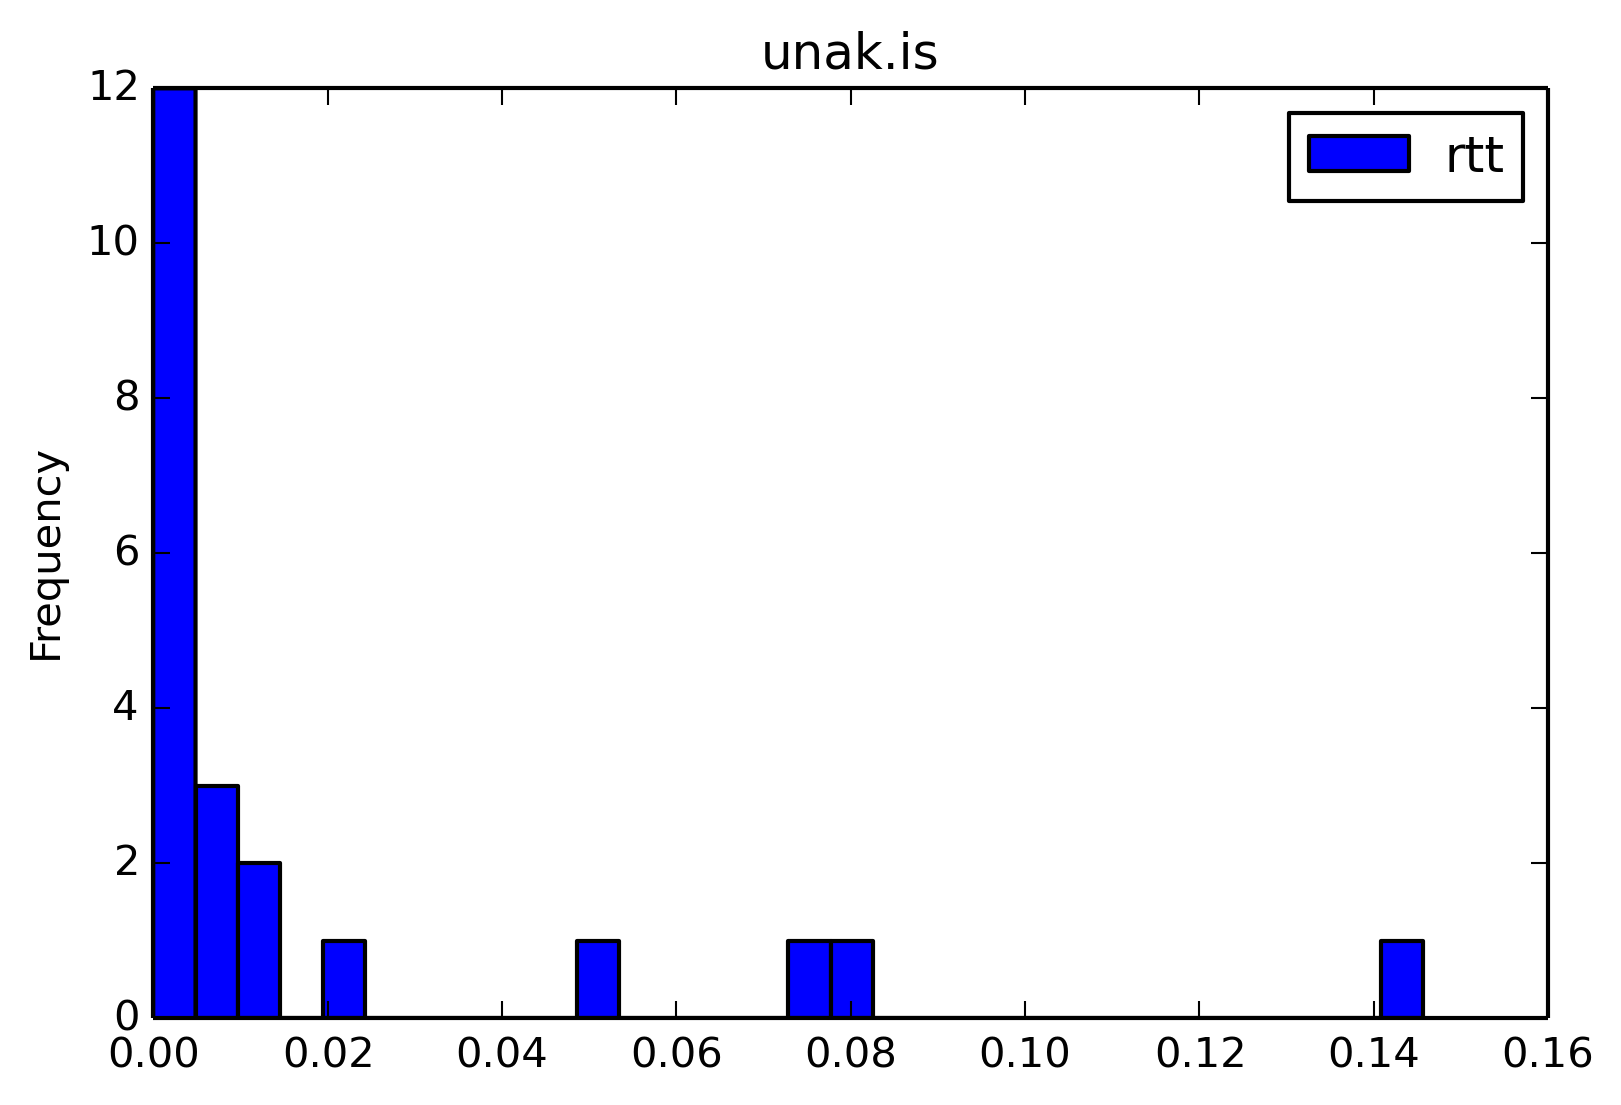
\includegraphics[width=0.45\textwidth]{histogramas_rtt/unak-is.png}
  \caption{RTT entre saltos}
  \label{entropia-s}
\end{figure}

\begin{center}
\captionof{table}{Outliers para unak.is}
\scalebox{0.8}{
\begin{tabular}{llllr}
\toprule
        &    &               &    &      rtt \\
host & ttl & ip & cc &          \\
\midrule
unak.is & 9  & 67.16.159.37 & US &  3.44859 \\
\bottomrule
\end{tabular}}
\end{center}

\begin{figure}[H]
  \centering
    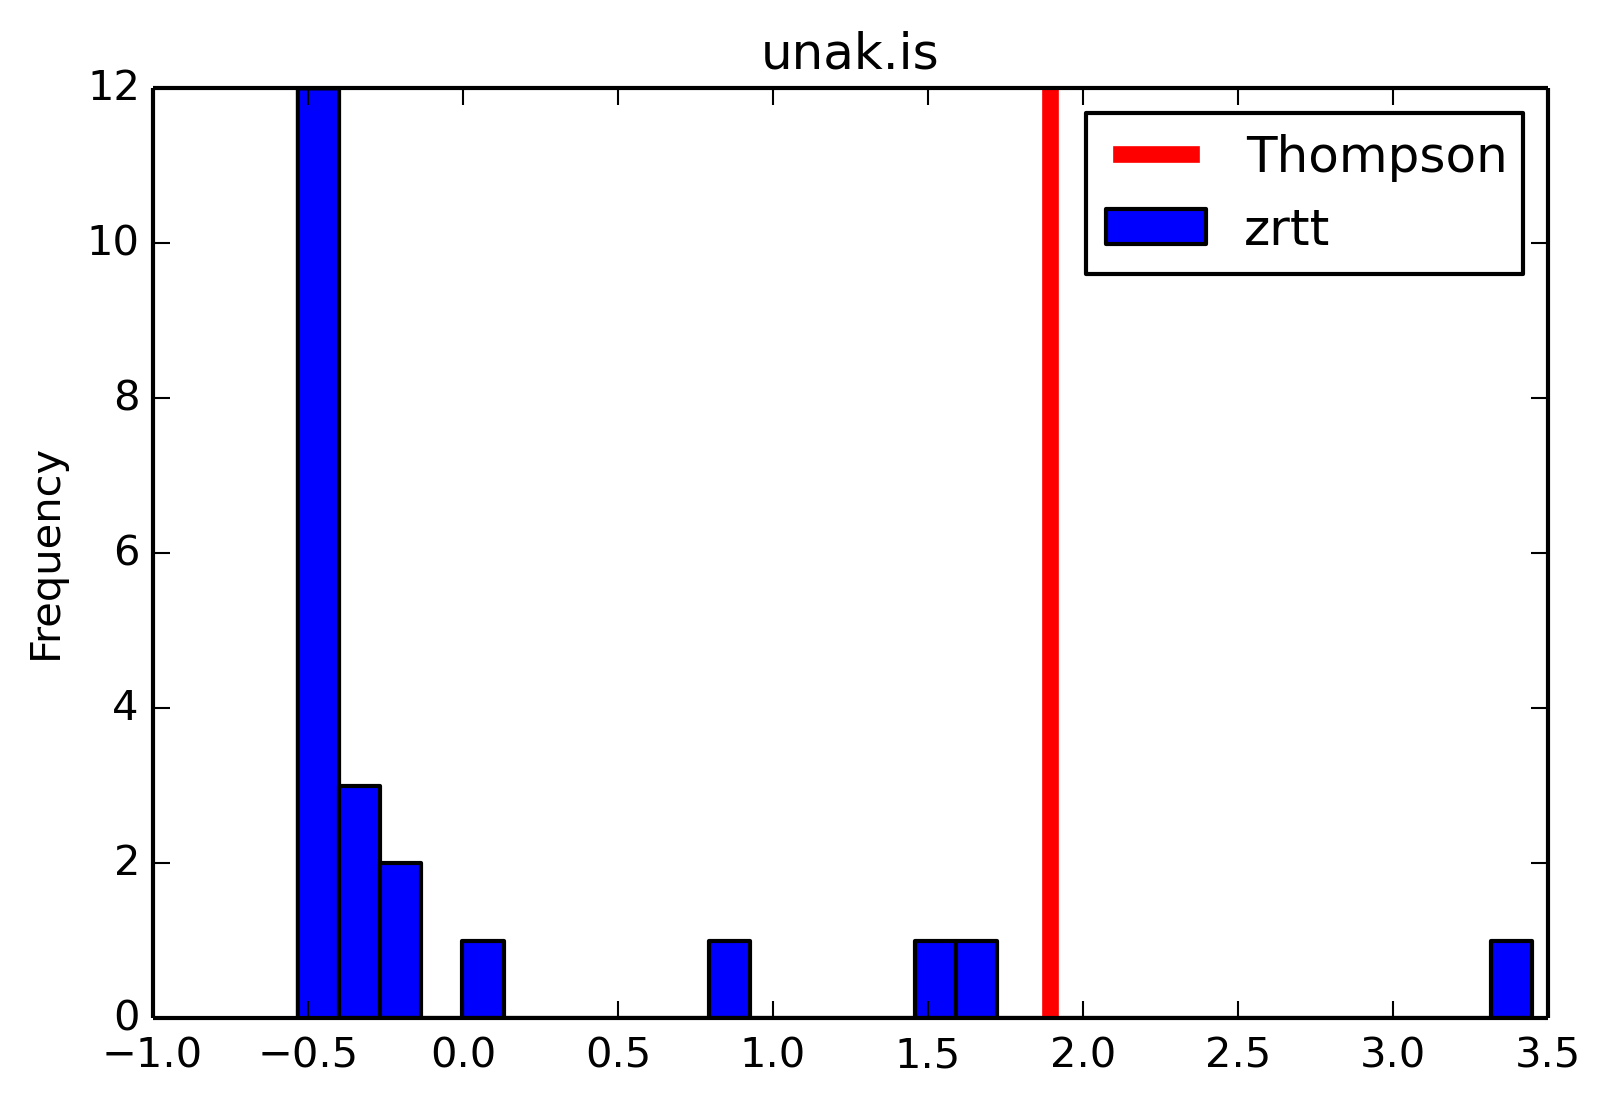
\includegraphics[width=0.45\textwidth]{histogramas_thompson/unak-is.png}
  \caption{RTT }
  \label{entropia-s}
\end{figure}

\begin{figure}[H]
  \centering
    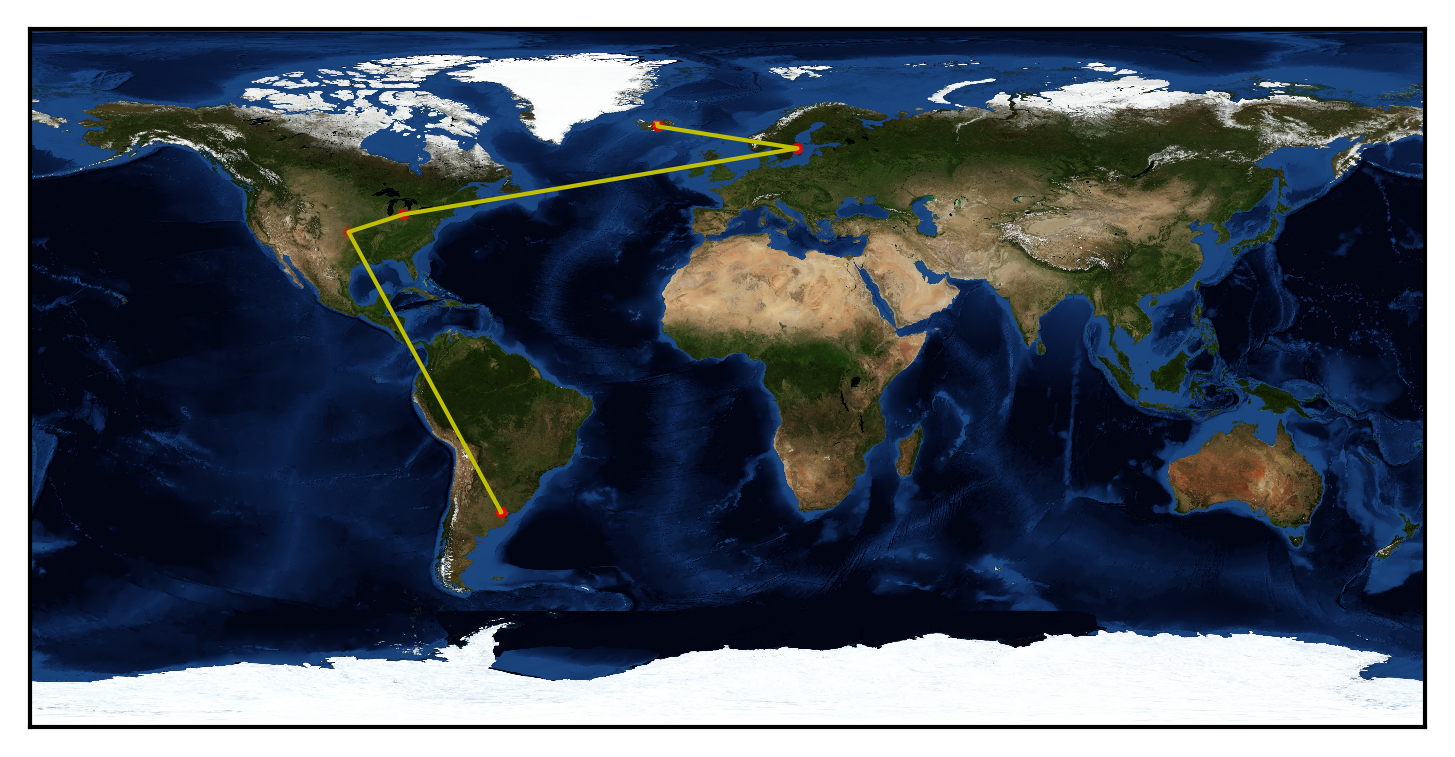
\includegraphics[width=0.45\textwidth]{grafico-rutas/unak-is.png}
  \caption{Gráfico de la ruta}
  \label{entropia-s}
\end{figure}



\subsection{Servidor unis.no}
\begin{center}
\captionof{table}{rtt promedios entre saltos para unis.no}
\scalebox{0.8}{
\begin{tabular}{llllr}
\toprule
        &    &                &    &       rtt \\
host & ttl & ip & cc &           \\
\midrule
unis.no & 1  & empty & empty &  0.000000 \\
        & 2  & empty & empty &  0.000000 \\
        & 3  & empty & empty &  0.000000 \\
        & 4  & empty & empty &  0.000000 \\
        & 5  & 200.89.161.97 & AR &  0.072603 \\
        & 6  & 200.89.165.1 & AR &  0.005187 \\
        & 7  & 200.89.165.250 & AR &  0.003868 \\
        & 8  & empty & empty &  0.000000 \\
        & 9  & 64.215.102.181 & US &  0.137360 \\
        & 10 & 64.57.20.73 & US &  0.008581 \\
        & 11 & 64.57.20.34 & US &  0.006402 \\
        & 12 & 64.57.20.37 & US &  0.008664 \\
        & 13 & empty & empty &  0.000000 \\
        & 14 & 109.105.97.142 & SE &  0.085971 \\
        & 15 & 109.105.97.138 & SE &  0.010124 \\
        & 16 & 109.105.102.66 & SE &  0.019075 \\
        & 17 & 109.105.102.67 & SE &  0.012499 \\
        & 18 & 128.39.255.121 & NO &  0.004408 \\
        & 19 & 128.39.255.47 & NO &  0.019374 \\
        & 20 & 128.39.255.211 & NO &  0.009346 \\
        & 21 & 128.39.255.19 & NO &  0.006287 \\
        & 22 & 128.39.254.85 & NO &  0.008778 \\
        & 23 & 128.39.47.158 & NO &  0.008459 \\
        & 24 & 158.39.149.250 & NO &  0.005062 \\
\bottomrule
\end{tabular}}
\end{center}

\begin{center}
\begin{tabular}{p{6.5cm}r}
Porcentaje de saltos que no responden los $Time$ $exceeded$: & \textbf{25\%} \\ \\ 
Largo de la ruta en términos de saltos que responden: &\textbf{18 saltos} \\ \\
Cantidad de enlaces intercontinentales: & \textbf{1} \\ \\
Cantidad de outliers según el método de Cimbala: & \textbf{2} \\ \\
\end{tabular}
\end{center}

No se corresponden los enlaces con los outliers.

\begin{figure}[H]
  \centering
    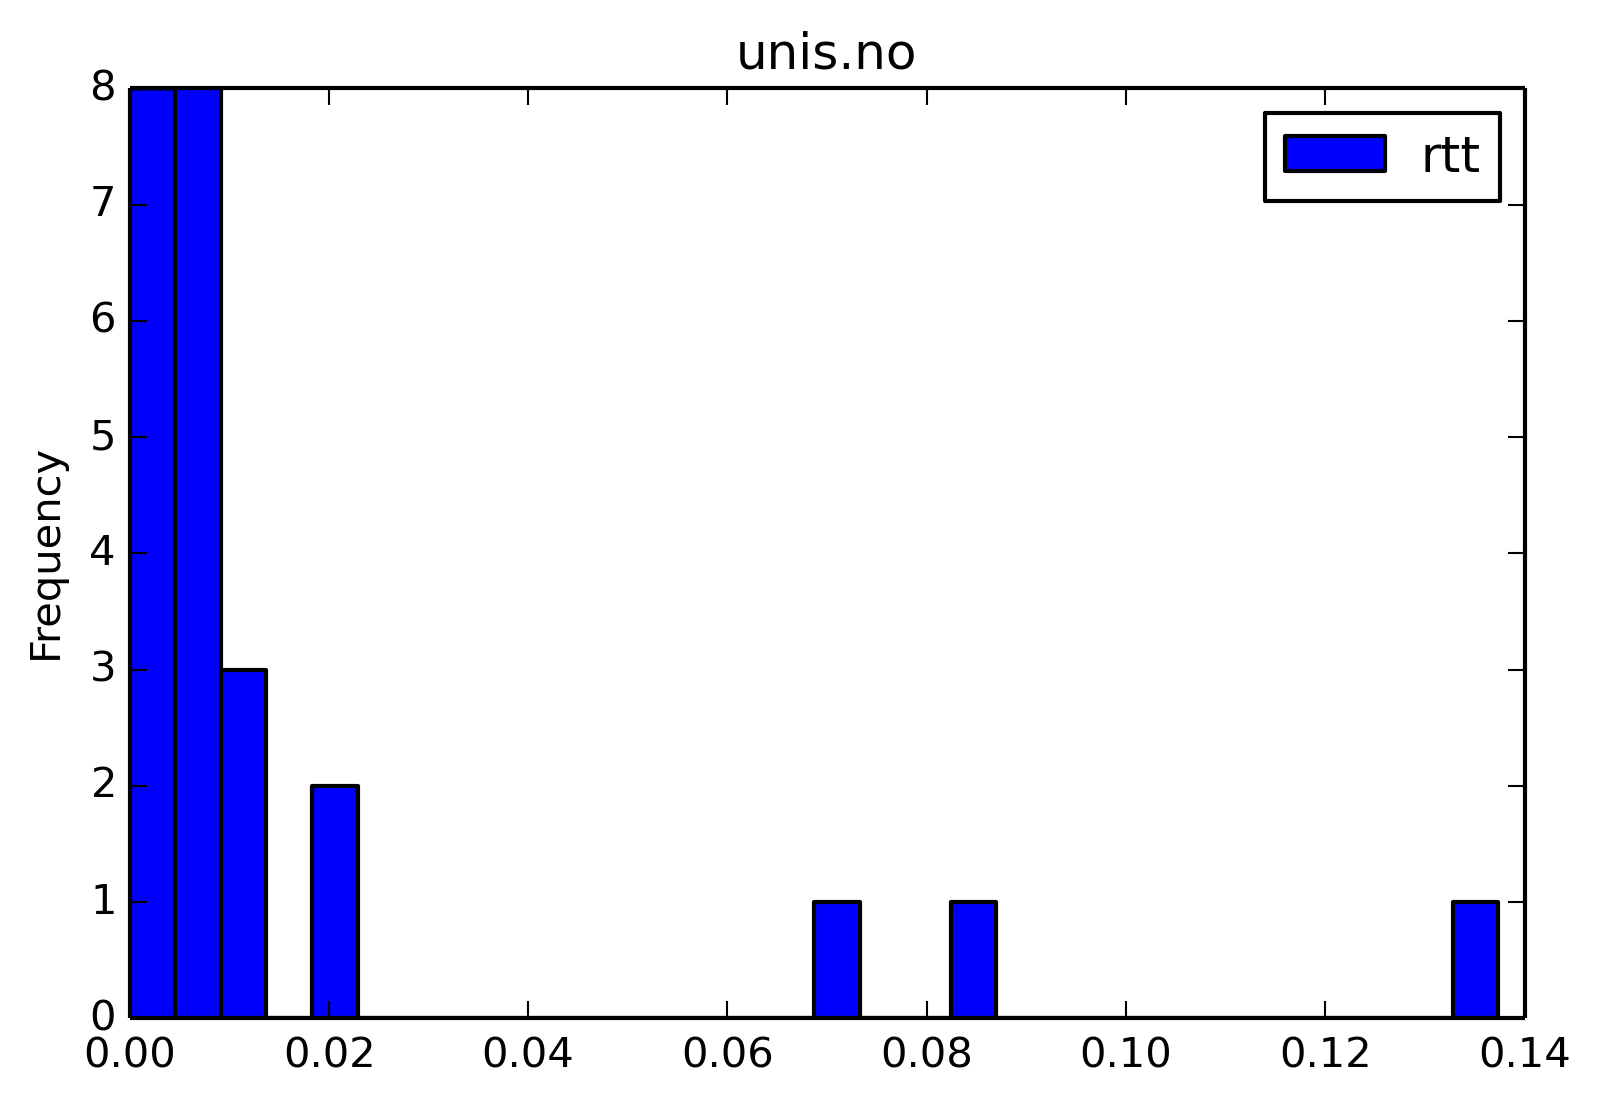
\includegraphics[width=0.45\textwidth]{histogramas_rtt/unis-no.png}
  \caption{RTT entre saltos}
  \label{entropia-s}
\end{figure}

\begin{center}\captionof{table}{Outliers para unis.no}
\scalebox{0.8}{
\begin{tabular}{llllr}
\toprule
        &    &                &    &       rtt \\
host & ttl & ip & cc &           \\
\midrule
unis.no & 9  & 64.215.102.181 & US &  3.598609 \\
        & 14 & 109.105.97.142 & SE &  2.049258 \\
\bottomrule
\end{tabular}}

\end{center}

\begin{figure}[H]
  \centering
    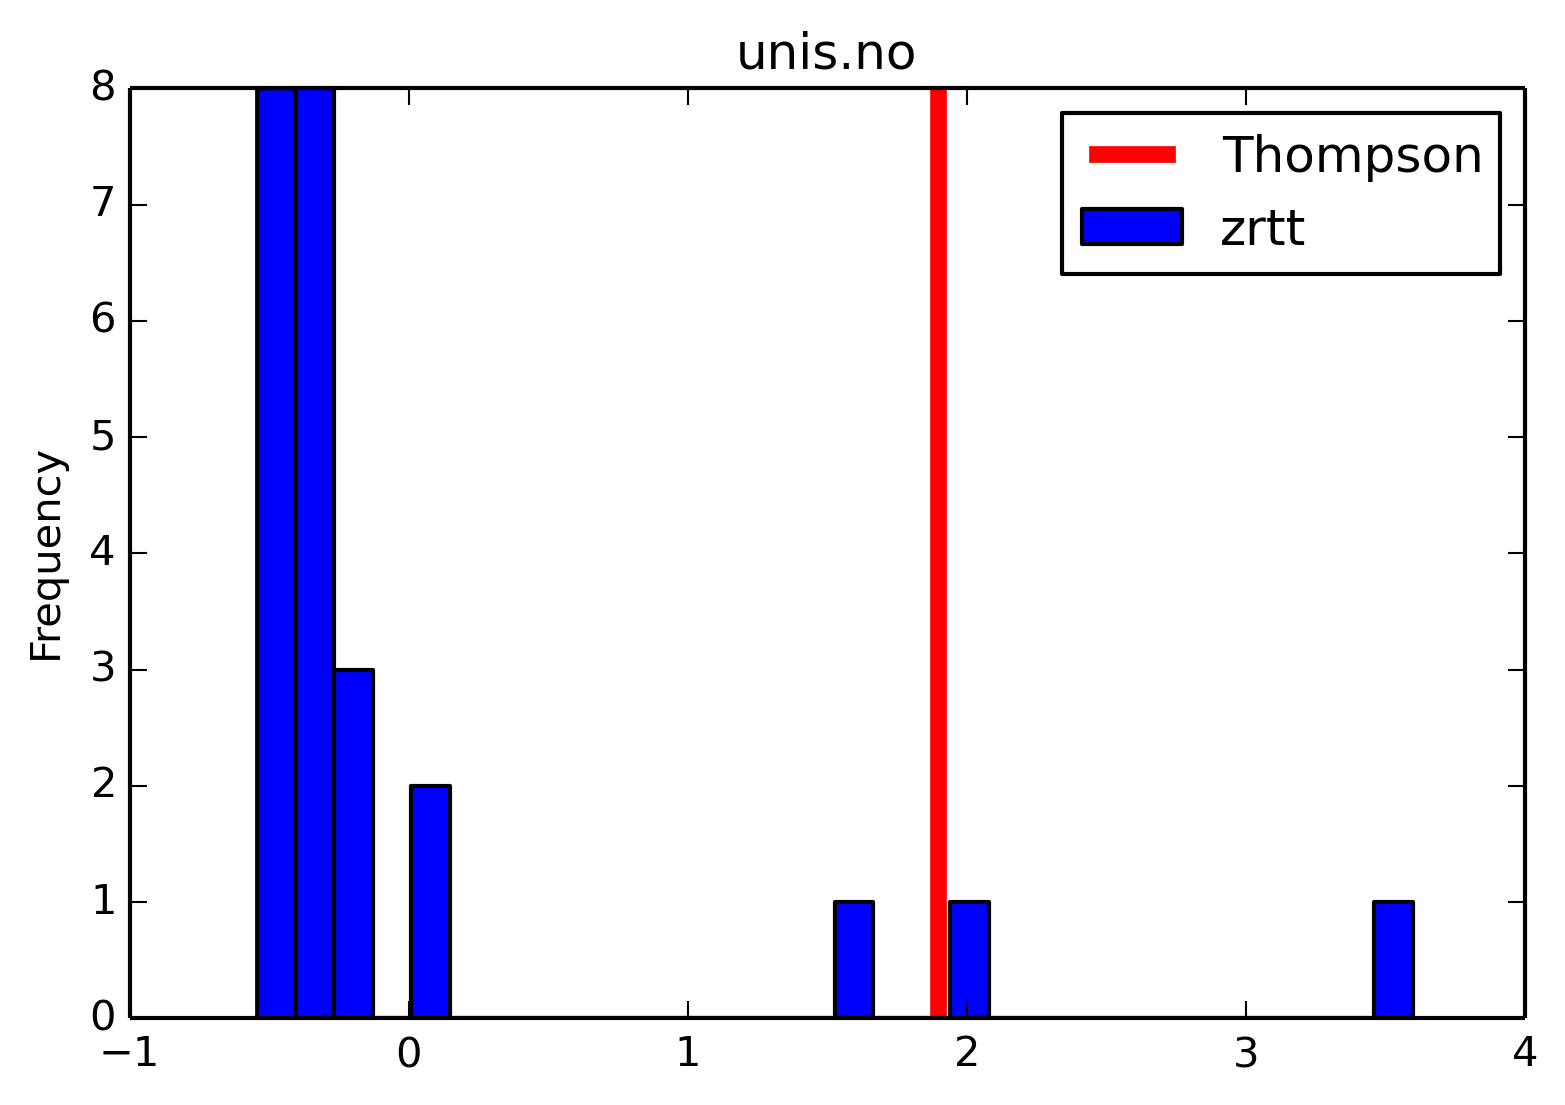
\includegraphics[width=0.45\textwidth]{histogramas_thompson/unis-no.png}
  \caption{RTTs Normailzados comparados con el valor Thompson}
  \label{entropia-s}
\end{figure}

\begin{figure}[H]
  \centering
    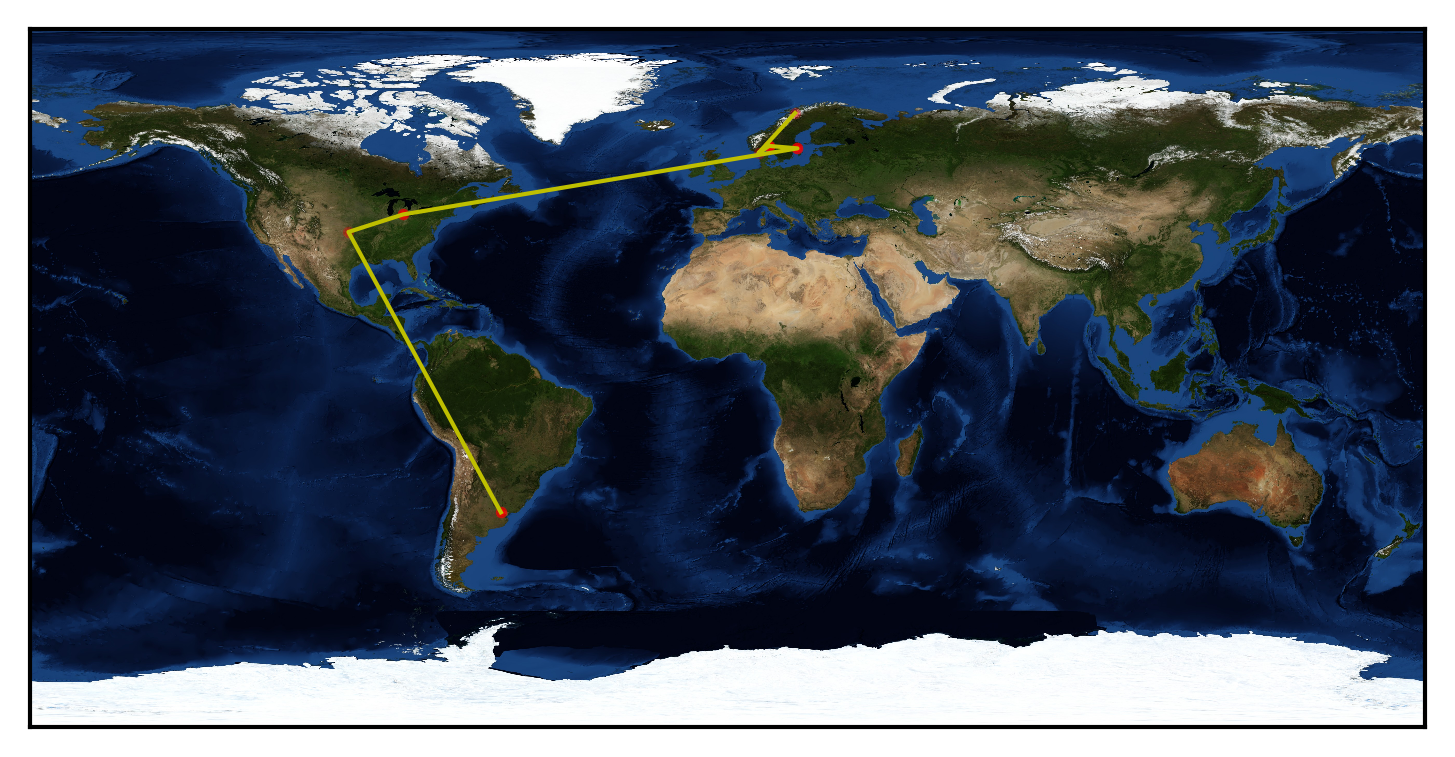
\includegraphics[width=0.45\textwidth]{grafico-rutas/unis-no.png}
  \caption{Gráfico de la ruta}
  \label{entropia-s}
\end{figure}




\subsection{Servidor www.fu-berlin.de}
\begin{center}
\captionof{table}{rtt promedios entre saltos para www.fu-berlin.de}
\scalebox{0.8}{
\begin{tabular}{llllr}
\toprule
                 &    &                &    &       rtt \\
host & ttl & ip & cc &           \\
\midrule
www.fu-berlin.de & 1  & empty & empty &  0.000000 \\
                 & 2  & empty & empty &  0.000000 \\
                 & 3  & empty & empty &  0.000000 \\
                 & 4  & empty & empty &  0.000000 \\
                 & 5  & 200.89.161.97 & AR &  0.076244 \\
                 & 6  & 200.89.165.197 & AR &  0.003247 \\
                 & 7  & 200.89.165.222 & AR &  0.005229 \\
                 & 8  & empty & empty &  0.000000 \\
                 & 9  & 67.17.94.249 & US &  0.131693 \\
                 & 10 & empty & empty &  0.000000 \\
                 & 11 & 4.69.154.73 & DE &  0.093868 \\
                 & 12 & 4.69.154.73 & DE &  0.011529 \\
                 & 13 & 212.162.4.6 & DE &  0.006355 \\
                 & 14 & 188.1.144.134 & DE &  0.014622 \\
                 & 15 & 188.1.234.174 & DE &  0.013845 \\
                 & 16 & 160.45.252.102 & DE &  0.009071 \\
                 & 17 & 130.133.99.102 & DE &  0.001297 \\
                 & 18 & 130.133.99.110 & DE&  0.004726 \\
                 & 19 & 160.45.170.10 & DE &  0.014093 \\
\bottomrule
\end{tabular}}

\end{center}

\begin{center}
\begin{tabular}{p{6.5cm}r}
Porcentaje de saltos que no responden los $Time$ $exceeded$: & \textbf{31\%} \\ \\ 
Largo de la ruta en términos de saltos que responden: &\textbf{13 saltos} \\ \\
Cantidad de enlaces intercontinentales: & \textbf{1} \\ \\
Cantidad de outliers según el método de Cimbala: & \textbf{2} \\ \\
\end{tabular}
\end{center}

No se corresponden los enlaces con los outliers.

\begin{figure}[H]
  \centering
    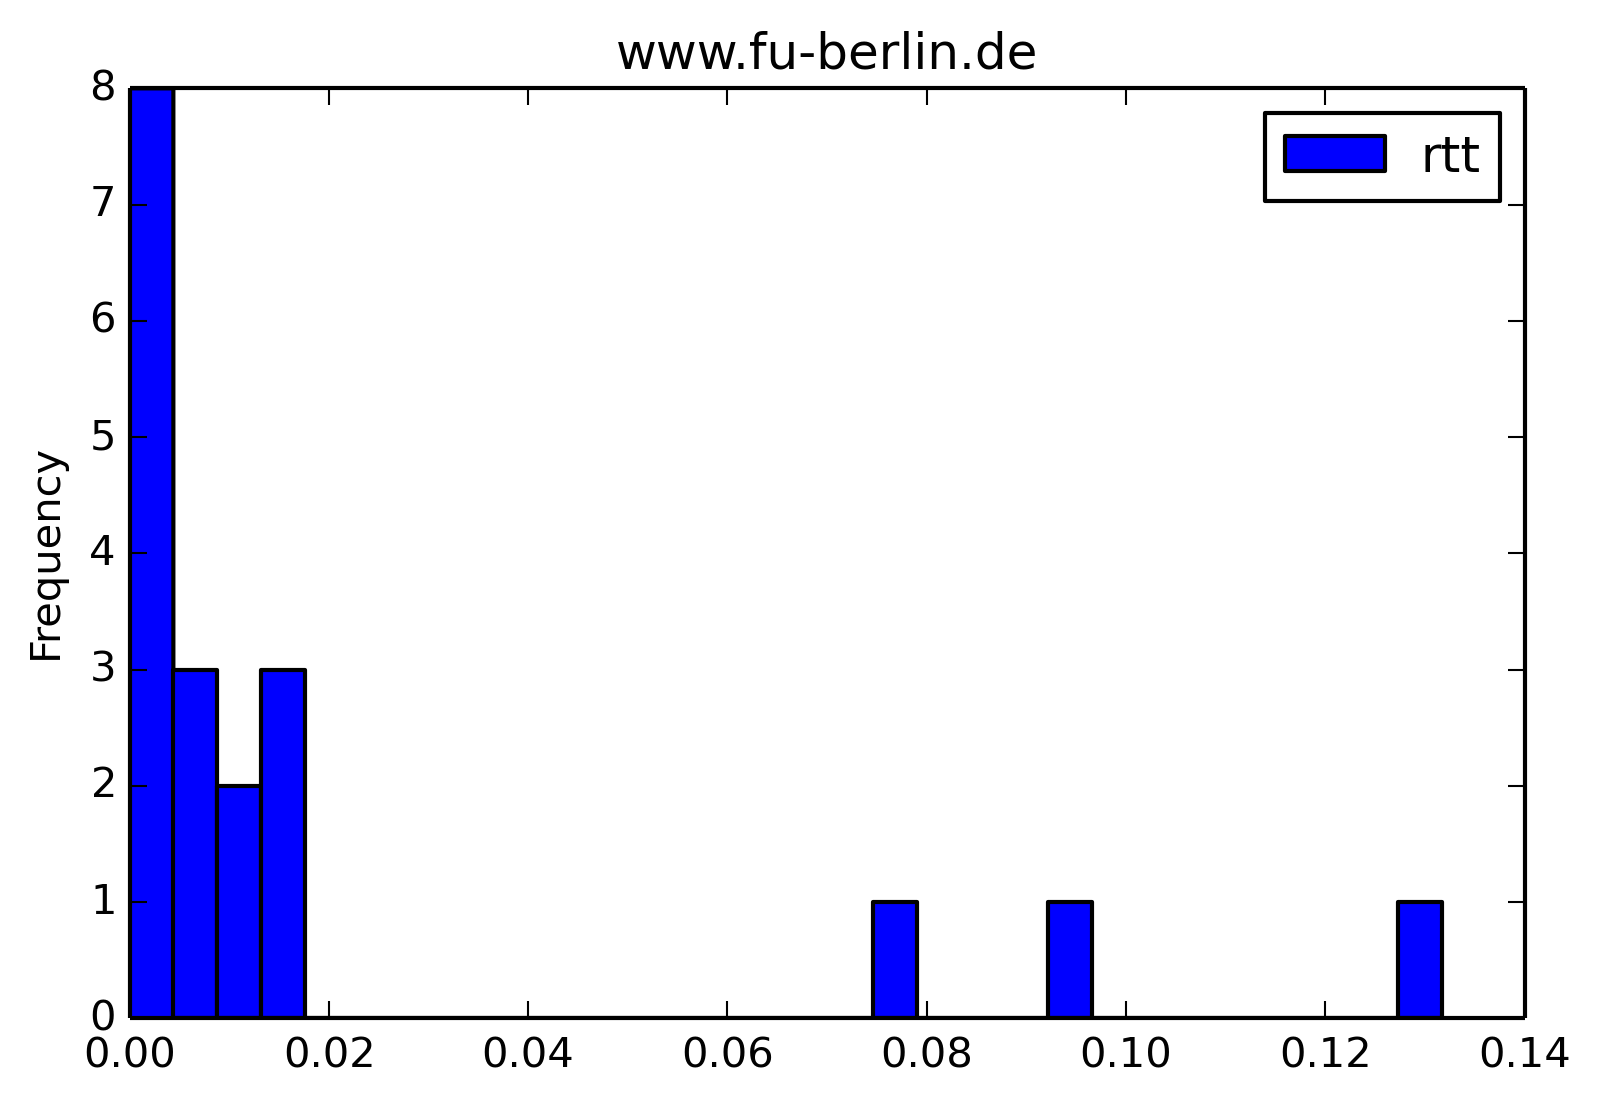
\includegraphics[width=0.45\textwidth]{histogramas_rtt/www-fu-berlin-de.png}
  \caption{RTT entre saltos}
  \label{entropia-s}
\end{figure}

\begin{center}
\captionof{table}{Outliers para www.fu-berlin.de}
\scalebox{0.8}{
\begin{tabular}{llllr}
\toprule
                 &    &                &    &       rtt \\
host & ttl & ip & cc &           \\
\midrule
www.fu-berlin.de & 9  & 67.17.94.249 & US &  2.985575 \\
                 & 11 & 4.69.154.73 &  DE &  1.971715 \\
\bottomrule
\end{tabular}}

\end{center}

\begin{figure}[H]
  \centering
    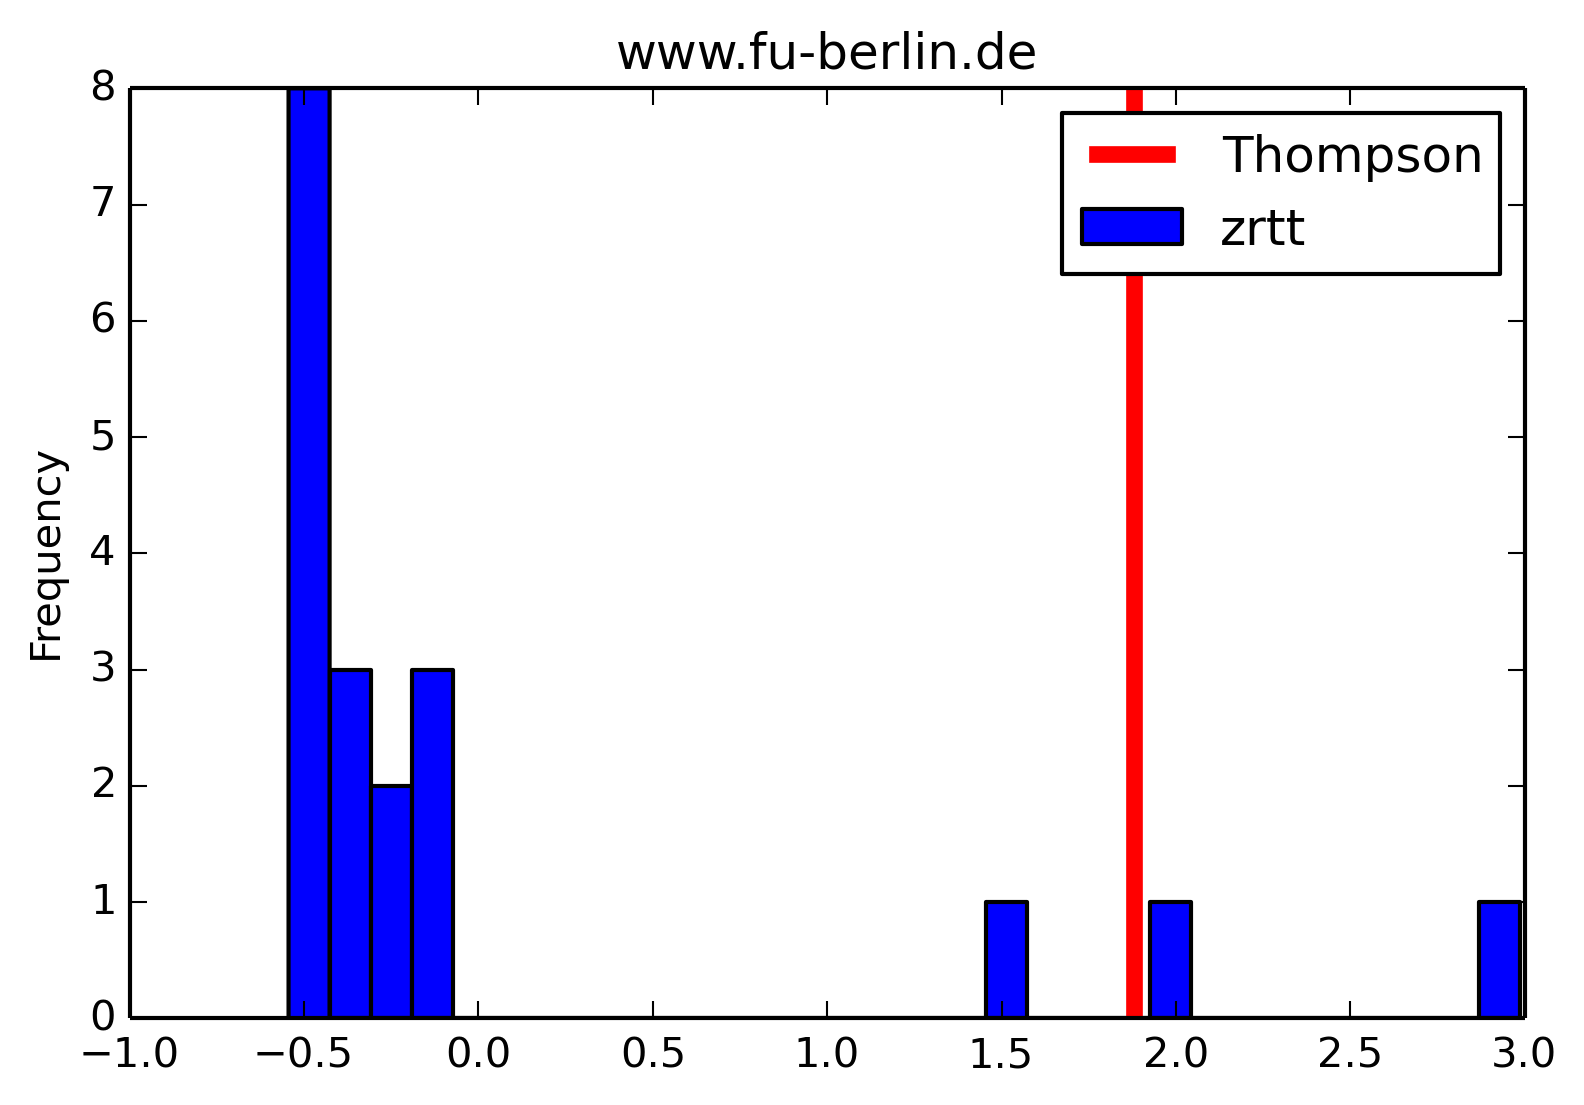
\includegraphics[width=0.45\textwidth]{histogramas_thompson/www-fu-berlin-de.png}
  \caption{RTTs Normailzados comparados con el valor Thompson}
  \label{entropia-s}
\end{figure}

\begin{figure}[H]
  \centering
    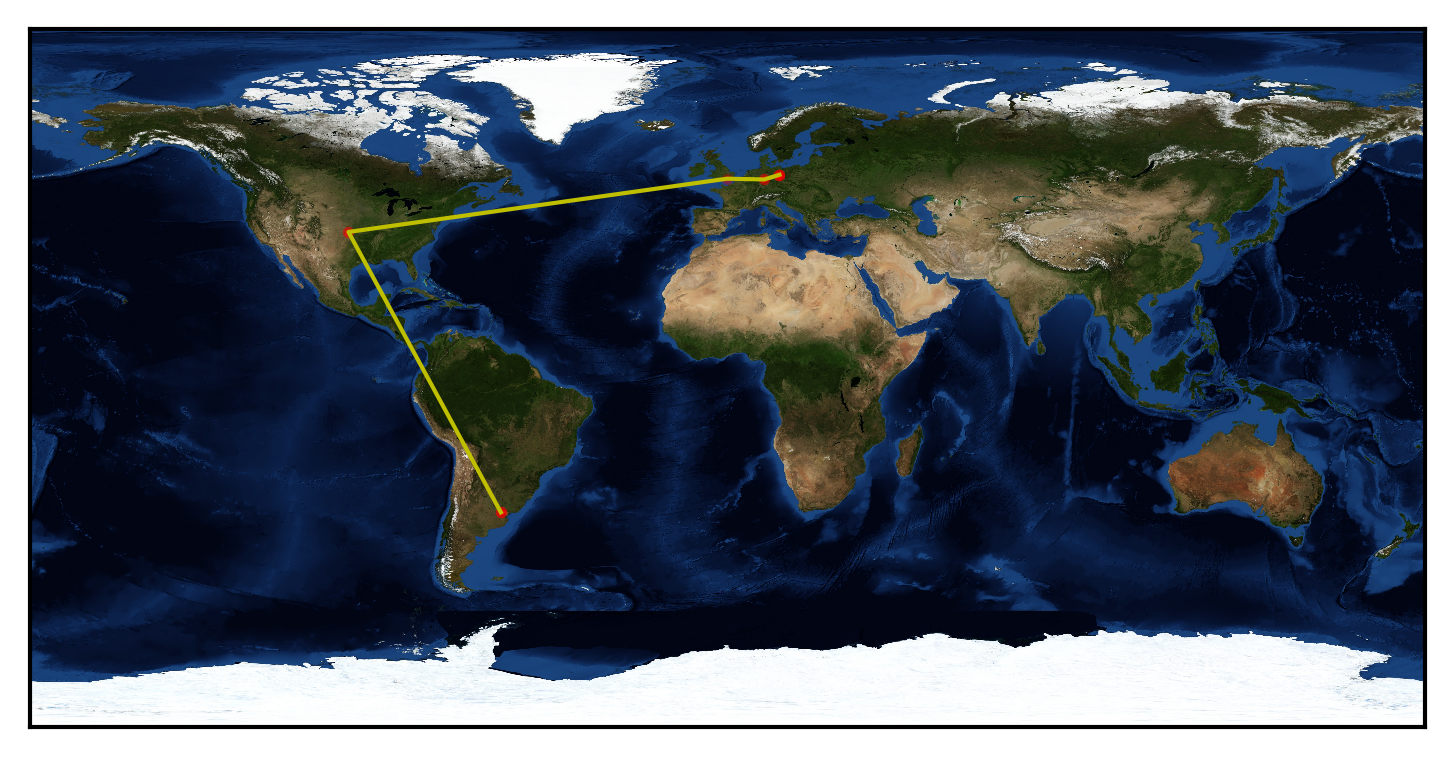
\includegraphics[width=0.45\textwidth]{grafico-rutas/www-fu-berlin-de.png}
  \caption{Gráfico de la ruta}
  \label{entropia-s}
\end{figure}




\subsection{Servidor www.kstu.kz}
\begin{center}
\captionof{table}{rtt promedios entre saltos para www.kstu.kz}
\scalebox{0.8}{
\begin{tabular}{llllr}
\toprule
            &    &               &    &       rtt \\
host & ttl & ip & cc &           \\
\midrule
www.kstu.kz & 1  & empty & empty &  0.000000 \\
            & 2  & empty & empty &  0.000000 \\
            & 3  & empty & empty &  0.000000 \\
            & 4  & empty & empty &  0.000000 \\
            & 5  & 200.89.161.145 & AR &  0.078752 \\
            & 6  & 200.89.165.150 & AR &  0.008279 \\
            & 7  & 185.70.203.20 & IT &  0.004113 \\
            & 8  & 195.22.214.131 & IT&  0.249391 \\
            & 9  & 195.22.211.109 & IT&  0.013956 \\
            & 10 & empty & empty &  0.000000 \\
            & 11 & 195.190.98.142 & RU &  0.081555 \\
            & 12 & 46.227.189.38 & KZ &  0.003893 \\
            &    & empty & empty &  0.000000 \\
            & 13 & 80.241.35.198 & KZ &  0.014117 \\
            & 14 & 85.29.137.2 & KZ &  0.068915 \\
            & 15 & 85.29.137.233 & KZ &  0.005942 \\
\bottomrule
\end{tabular}}
\end{center}


\begin{center}
\begin{tabular}{p{6.5cm}r}
Porcentaje de saltos que no responden los $Time$ $exceeded$: & \textbf{40\%} \\ \\ 
Largo de la ruta en términos de saltos que responden: &\textbf{15 saltos} \\ \\
Cantidad de enlaces intercontinentales: & \textbf{1} \\ \\
Cantidad de outliers según el método de Cimbala: & \textbf{1} \\ \\
\end{tabular}
\end{center}


\begin{figure}[H]
  \centering
    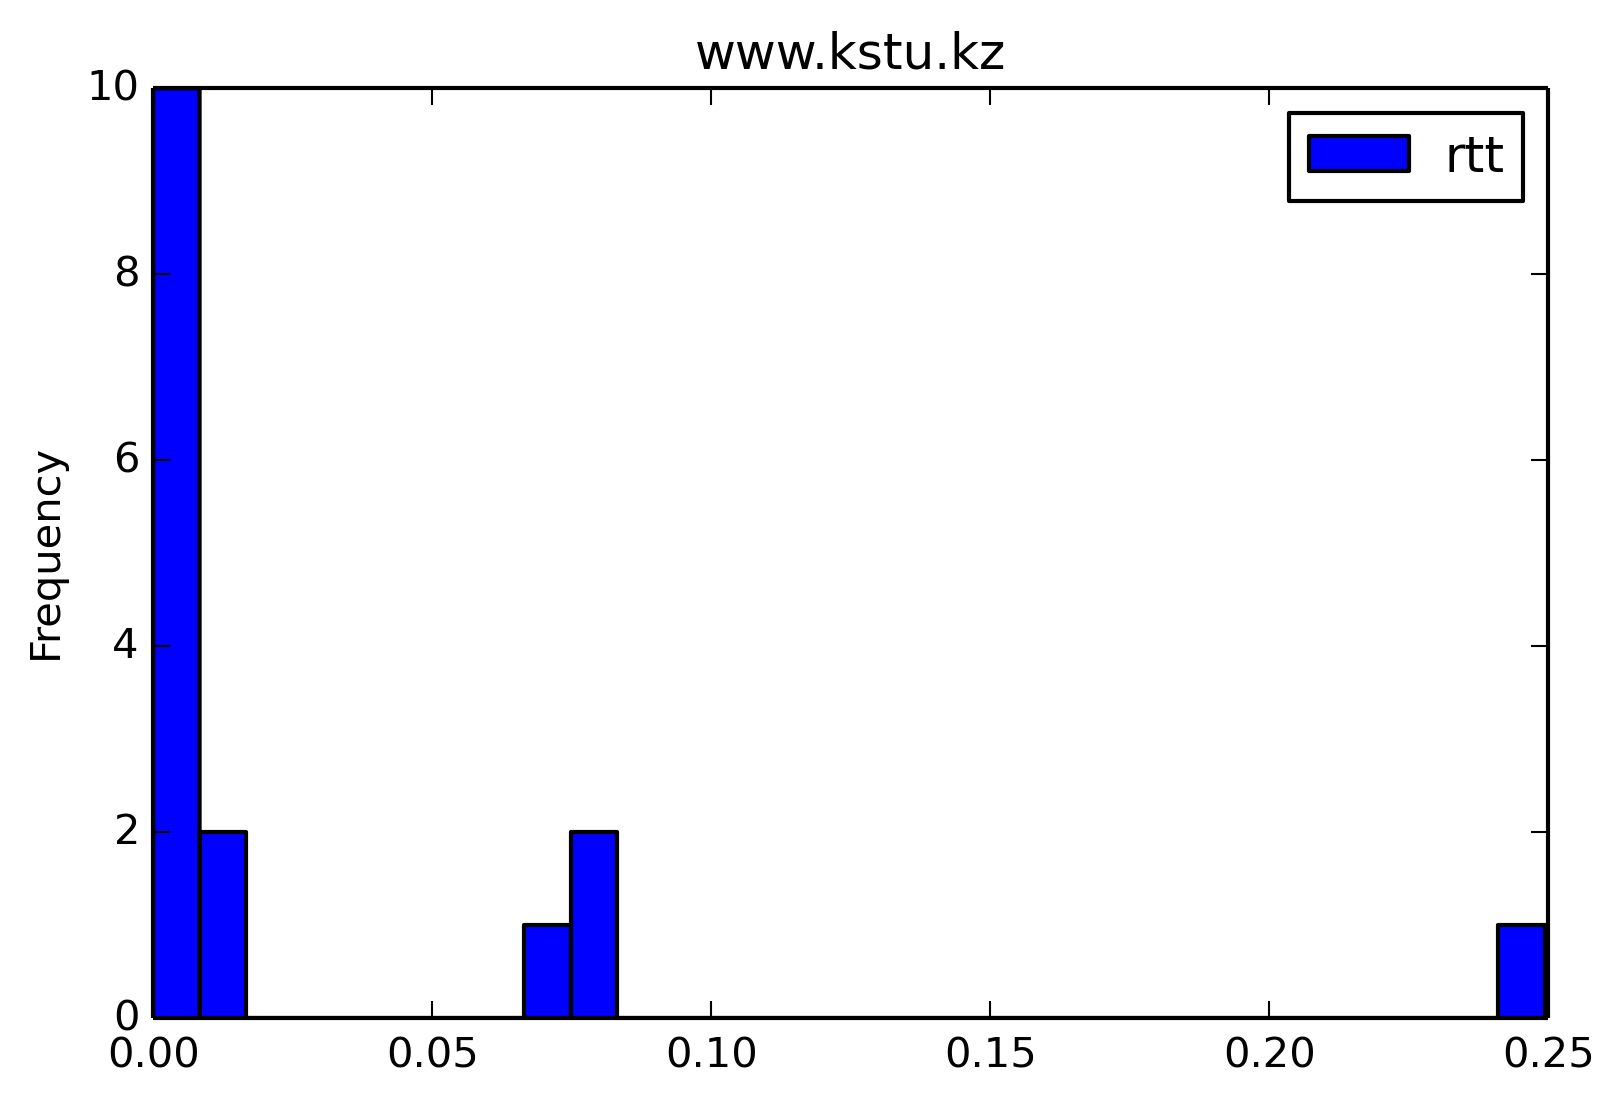
\includegraphics[width=0.45\textwidth]{histogramas_rtt/www-kstu-kz.png}
  \caption{RTT entre saltos}
  \label{entropia-s}
\end{figure}

\begin{center}
\captionof{table}{Outliers para www.kstu.kz}
\scalebox{0.8}{
\begin{tabular}{llllr}
\toprule
            &    &               &    &       rtt \\
host & ttl & ip & cc &           \\
\midrule
www.kstu.kz & 8  & 195.22.214.131 & IT &  3.342247 \\
\bottomrule
\end{tabular}}
\end{center}


\begin{figure}[H]
  \centering
    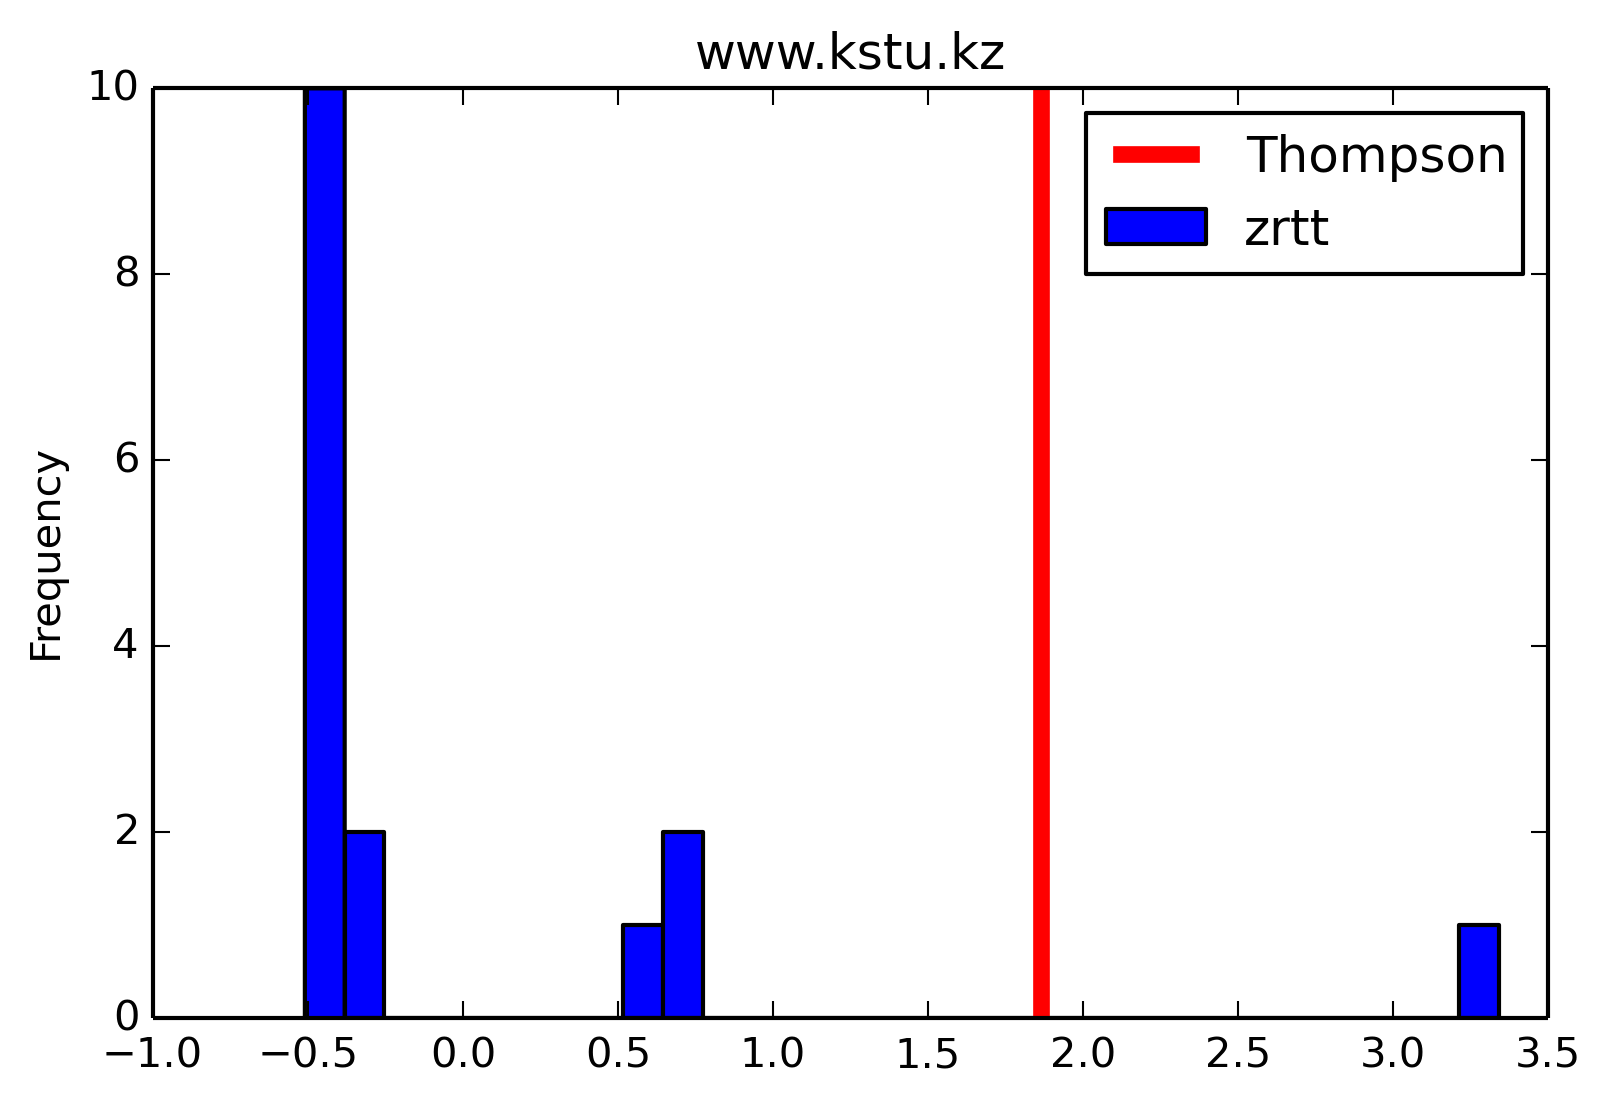
\includegraphics[width=0.45\textwidth]{histogramas_thompson/www-kstu-kz.png}
  \caption{RTTs Normailzados comparados con el valor Thompson}
  \label{entropia-s}
\end{figure}

\begin{figure}[H]
  \centering
    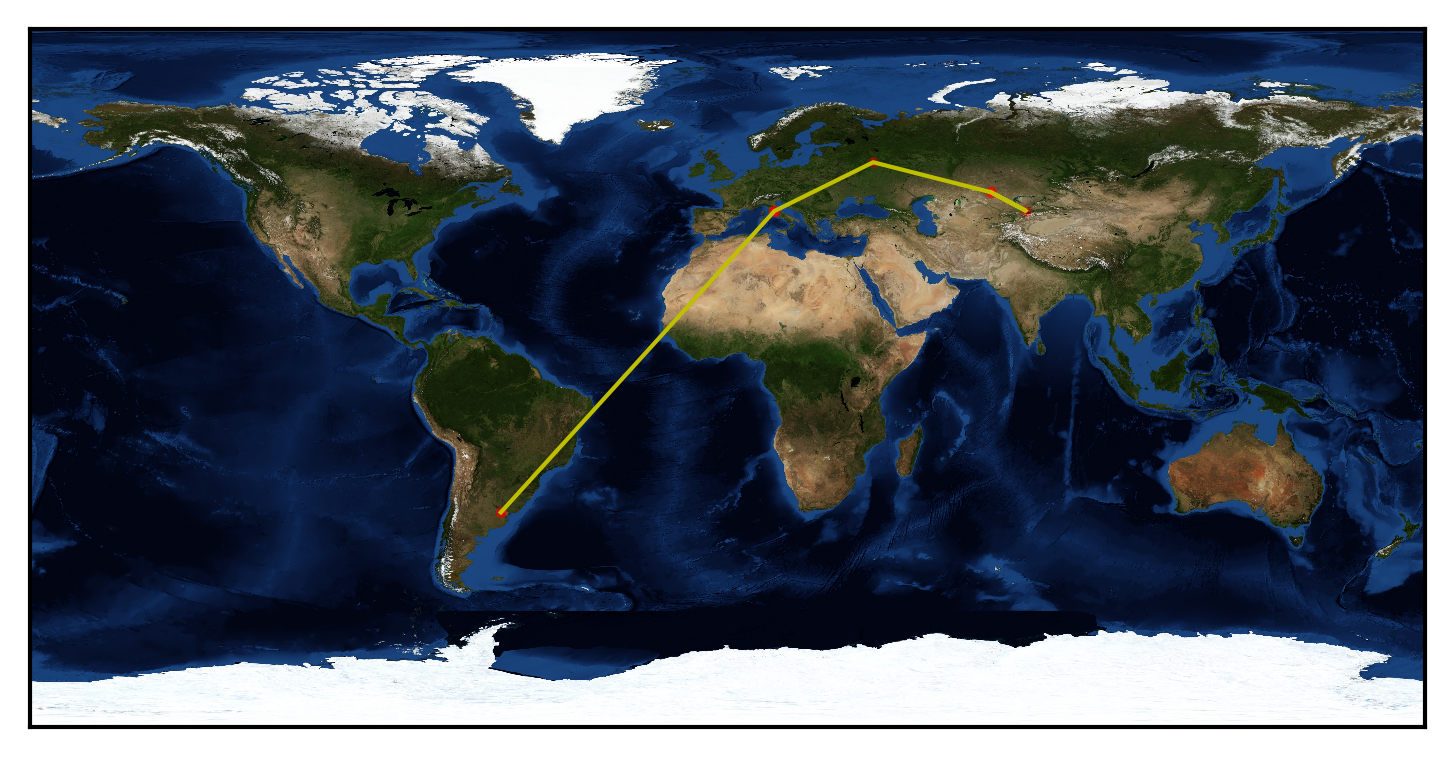
\includegraphics[width=0.45\textwidth]{grafico-rutas/www-kstu-kz.png}
  \caption{Gráfico de la ruta}
  \label{entropia-s}
\end{figure}




\subsection{Servidor www.uq.edu.au}
\begin{center}
\captionof{table}{rtt promedios entre saltos para www.uq.edu.au}
\scalebox{0.8}{
\begin{tabular}{llllr}
\toprule
              &    &                &    &       rtt \\
host & ttl & ip & cc &           \\
\midrule
www.uq.edu.au & 1  & empty & empty &  0.000000 \\
              & 2  & empty & empty &  0.000000 \\
              & 3  & empty & empty &  0.000000 \\
              & 4  & empty & empty &  0.000000 \\
              & 5  & 200.89.161.81 & AR &  0.069609 \\
              & 6  & 200.89.165.1 & AR &  0.005534 \\
              & 7  & 200.89.165.250 & AR &  0.007442 \\
              & 8  & empty & empty &  0.000000 \\
              & 9  & 67.17.94.249 & US &  0.121653 \\
              & 10 & empty & empty &  0.000000 \\
              & 11 & empty & empty &  0.000000 \\
              & 12 & 4.68.127.54 & US &  0.011813 \\
              & 13 & 129.250.4.250 & US &  0.008370 \\
              & 14 & 129.250.2.219 & US &  0.027036 \\
              & 15 & 129.250.7.69 & US &  0.015778 \\
              & 16 & 129.250.3.123 & US &  0.008138 \\
              & 17 & 204.1.253.166 & US &  0.028387 \\
              & 18 & 202.158.194.172 & AU &  0.139608 \\
              & 19 & 113.197.15.68 & AU &  0.002438 \\
              & 20 & 113.197.15.66 & AU &  0.006682 \\
              & 21 & 113.197.15.152 & AU &  0.023330 \\
              & 22 & 113.197.15.4 & AU &  0.011024 \\
              & 23 & 113.197.15.7 & AU &  0.015266 \\
              & 24 & 113.197.15.34 & AU &  0.003360 \\
              & 25 & 138.44.129.46 & AU &  0.009573 \\
              & 26 & 130.102.159.1 & AU &  0.021310 \\
              & 27 & 130.102.0.242 & AU &  0.007072 \\
              & 28 & 130.102.82.63 & AU &  0.005245 \\
              & 29 & 130.102.131.70 & AU &  0.004558 \\
\bottomrule
\end{tabular}}
\end{center}


\begin{center}
\begin{tabular}{p{6.5cm}r}
Porcentaje de saltos que no responden los $Time$ $exceeded$: & \textbf{24\%} \\ \\ 
Largo de la ruta en términos de saltos que responden: &\textbf{22 saltos} \\ \\
Cantidad de enlaces intercontinentales: & \textbf{1} \\ \\
Cantidad de outliers según el método de Cimbala: & \textbf{2} \\ \\
\end{tabular}
\end{center}

\begin{figure}[H]
  \centering
    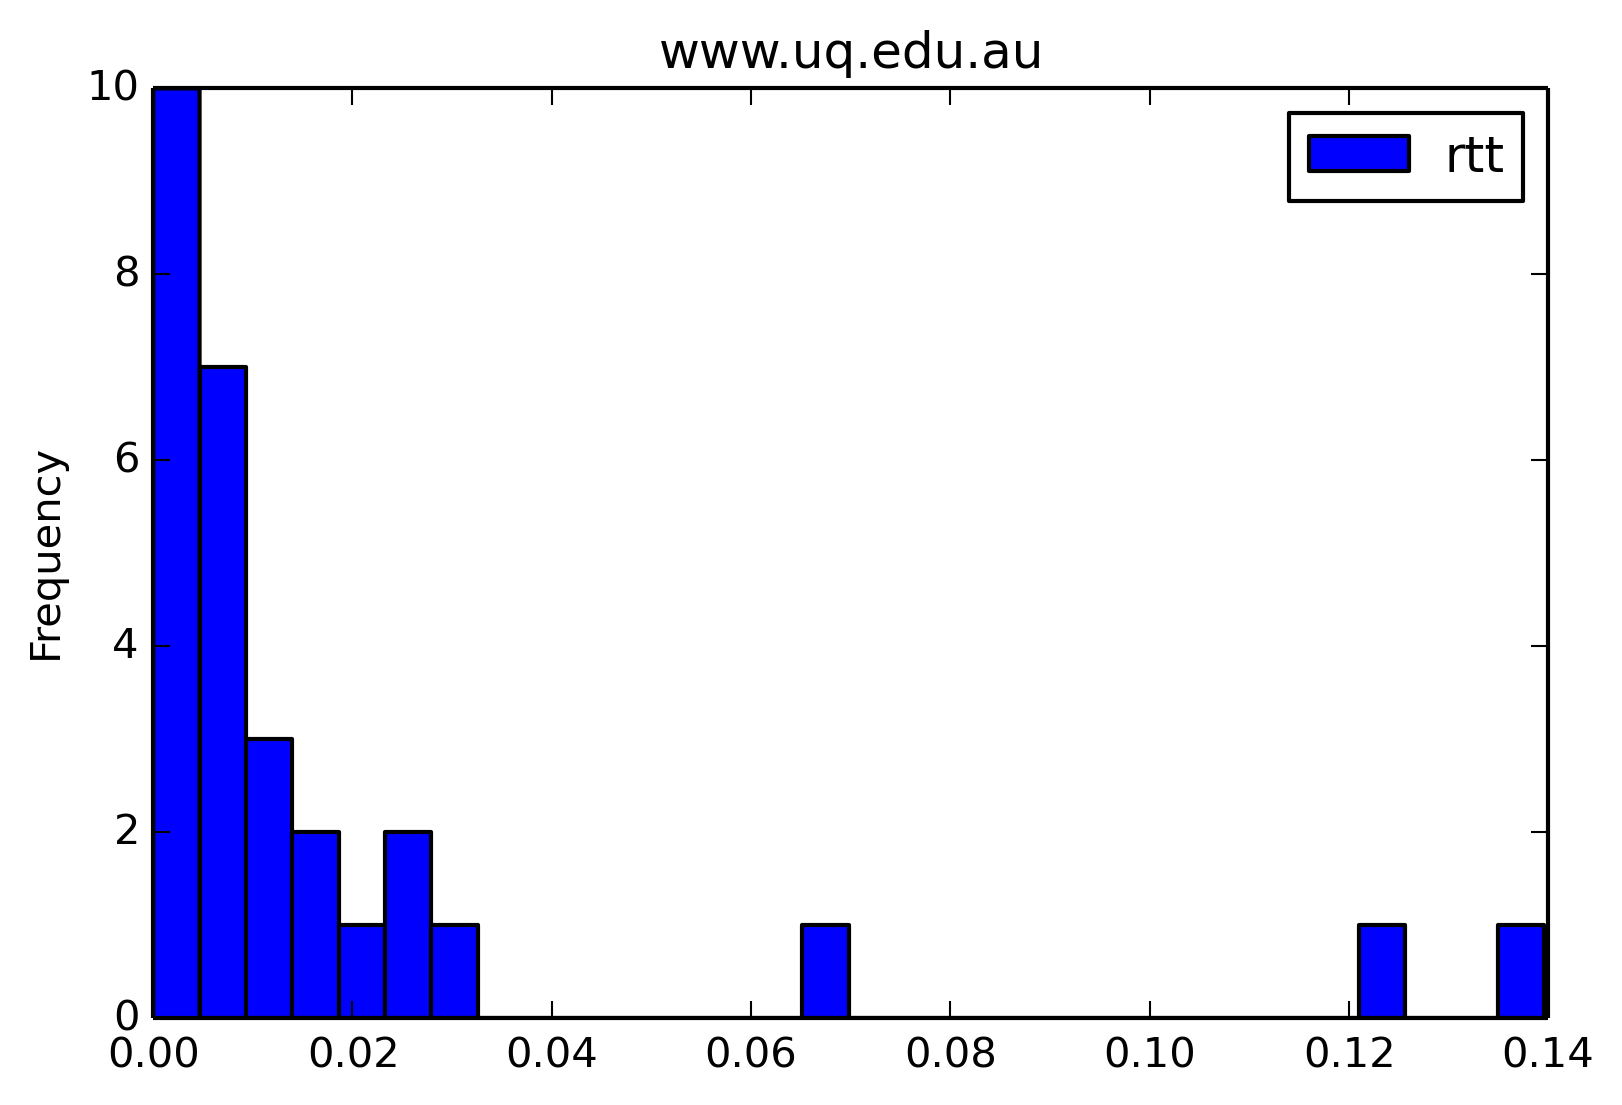
\includegraphics[width=0.45\textwidth]{histogramas_rtt/www-uq-edu-au.png}
  \caption{RTT entre saltos}
  \label{entropia-s}
\end{figure}

\begin{center}
\captionof{table}{Outliers para www.uq.edu.au}
\scalebox{0.8}{
\begin{tabular}{llllr}
\toprule
              &    &                &    &       rtt \\
host & ttl & ip & cc &           \\
\midrule
www.uq.edu.au & 9  & 67.17.94.249 & US &  3.018553 \\
              & 18 & 202.158.194.172 & AU &  3.546898 \\
\bottomrule
\end{tabular}}

\end{center}

\begin{figure}[H]
  \centering
    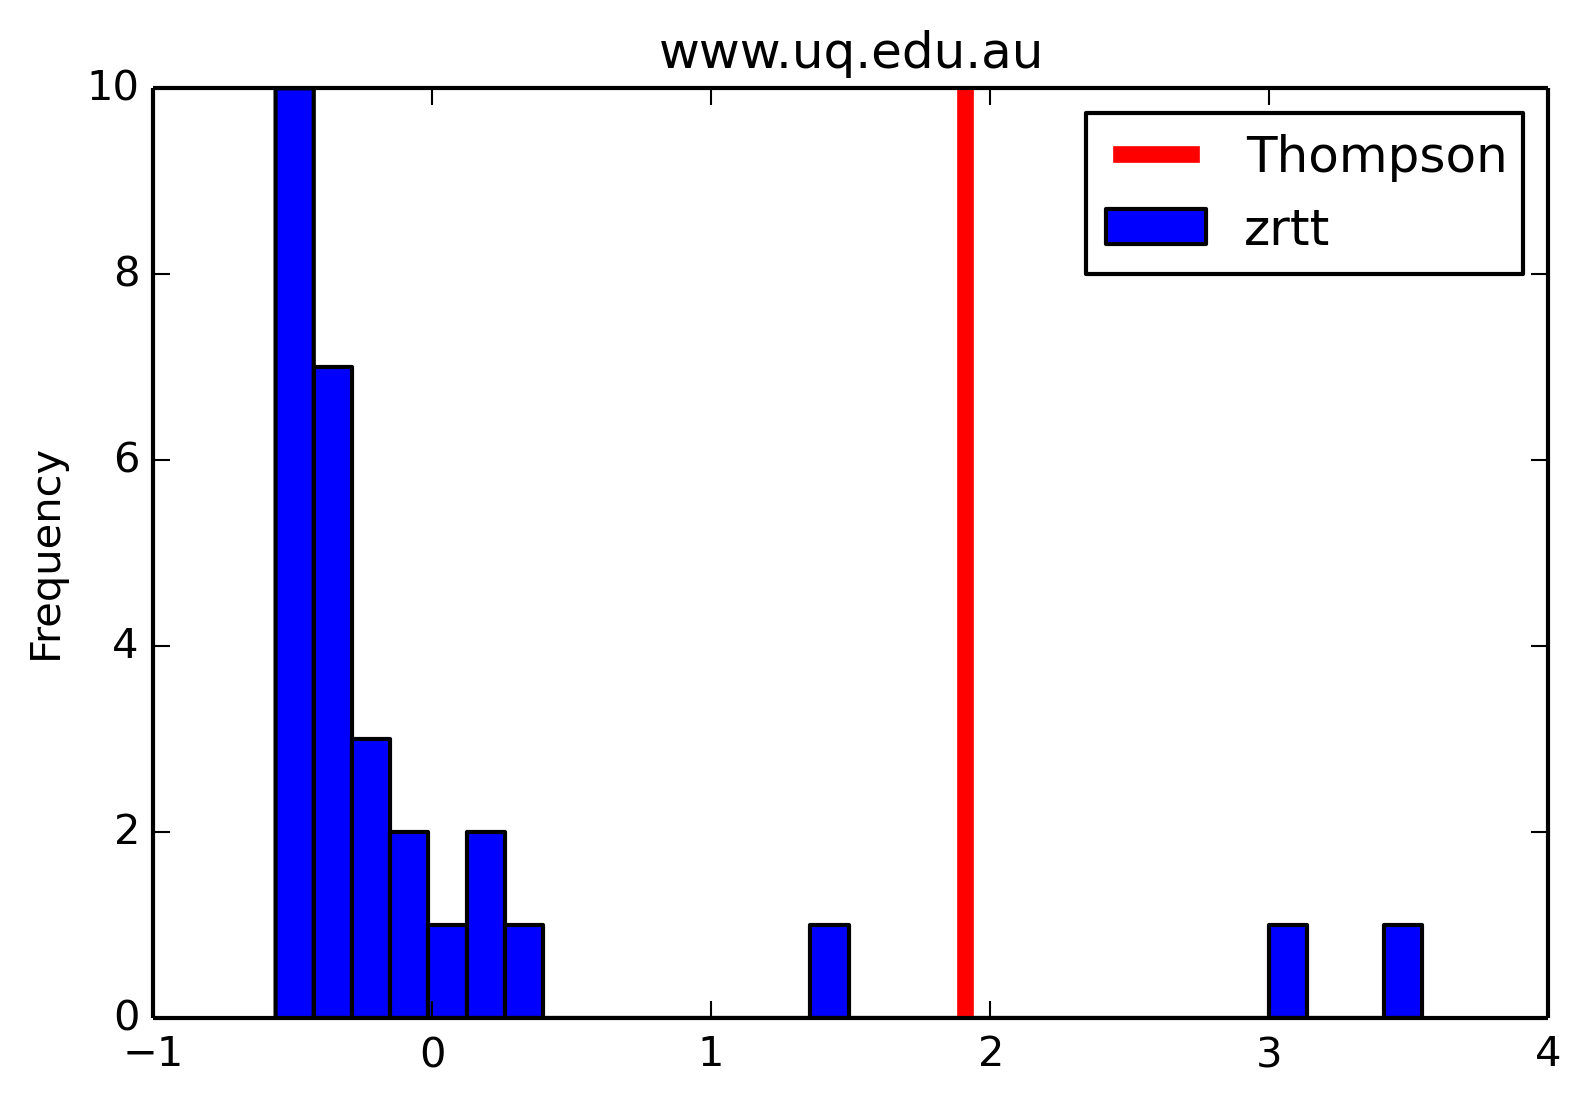
\includegraphics[width=0.45\textwidth]{histogramas_thompson/www-uq-edu-au.png}
  \caption{RTTs Normailzados comparados con el valor Thompson}
  \label{entropia-s}
\end{figure}

\begin{figure}[H]
  \centering
    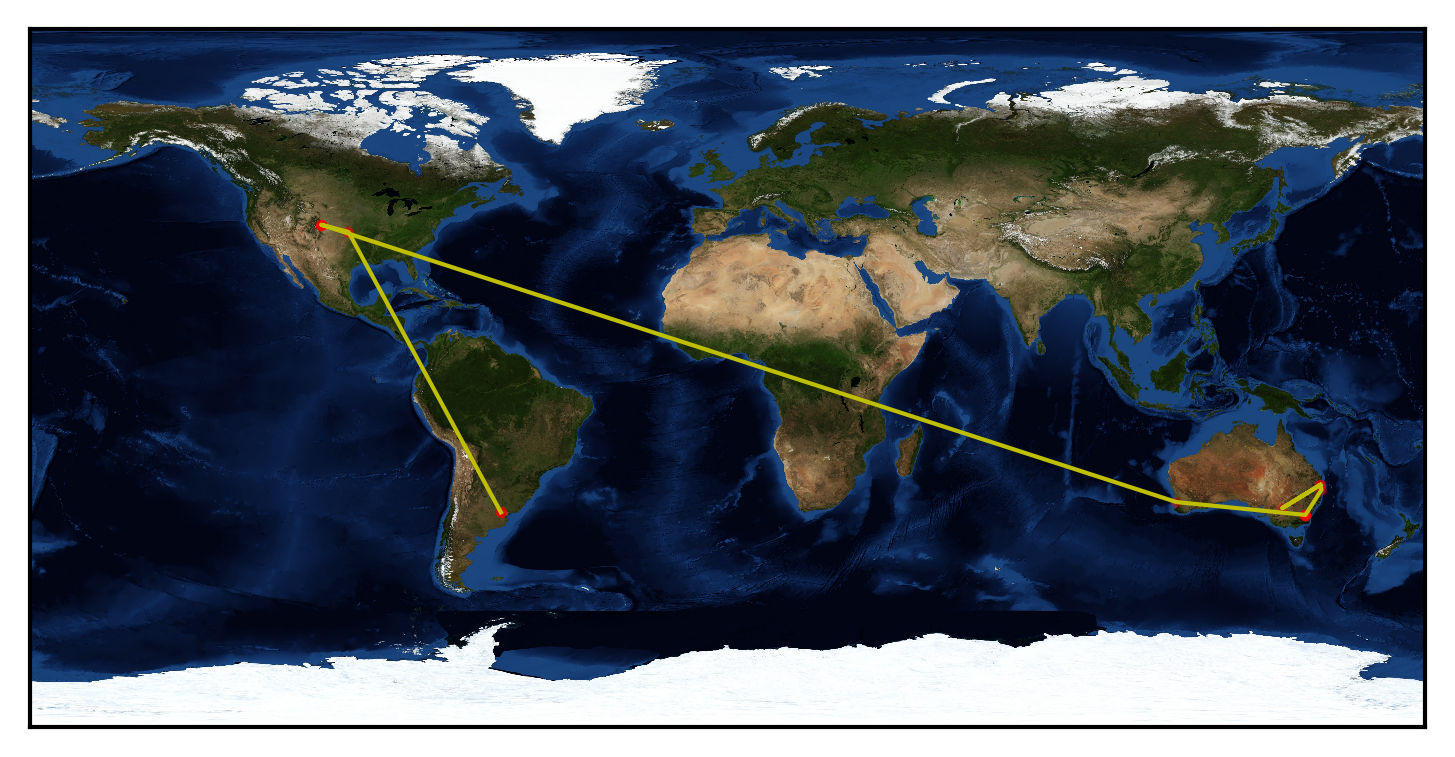
\includegraphics[width=0.45\textwidth]{grafico-rutas/www-uq-edu-au.png}
  \caption{Gráfico de la ruta}
  \label{entropia-s}
\end{figure}





\subsection{Servidor auckland.ac.nz}

\begin{center}
\captionof{table}{rtt promedios entre saltos para auckland.ac.nz}
\scalebox{0.8}{
\begin{tabular}{llllr}
\toprule
               &    &               &    &       rtt \\
host & ttl & ip & cc &           \\
\midrule
auckland.ac.nz & 1  & empty & empty &  0.000000 \\
               & 2  & empty & empty &  0.000000 \\
               & 3  & empty & empty &  0.000000 \\
               & 4  & empty & empty &  0.000000 \\
               & 5  & 200.89.161.77 & AR &  0.076270 \\
               & 6  & 200.89.165.197 & AR &  0.009660 \\
               & 7  & 200.89.165.222 & AR &  0.010555 \\
               & 8  & empty & empty &  0.000000 \\
               & 9  & 67.17.94.249 & US &  0.116990 \\
               & 10 & empty & empty &  0.000000 \\
               & 11 & empty & empty &  0.000000 \\
               & 12 & 4.68.127.54 & US &  0.008144 \\
               & 13 & 129.250.4.250 & US &  0.008747 \\
               & 14 & 129.250.2.219 & US &  0.026343 \\
               & 15 & 129.250.7.69 & US &  0.013037 \\
               & 16 & 129.250.3.123 & US &  0.005543 \\
               & 17 & 204.1.253.166 & US &  0.045089 \\
               & 18 & 202.158.194.172 & AU &  0.120172 \\
               & 19 & 182.255.119.139 & AU &  0.014907 \\
               & 20 & 210.7.39.251 & NZ &  0.014551 \\
               & 21 & 210.7.39.178 & NZ &  0.004857 \\
\bottomrule
\end{tabular}}
\end{center}

\begin{center}
\begin{tabular}{p{6.5cm}r}
Porcentaje de saltos que no responden los $Time$ $exceeded$: & \textbf{\%} \\ \\ 
Largo de la ruta en términos de saltos que responden: &\textbf{ saltos} \\ \\
Cantidad de enlaces intercontinentales: & \textbf{} \\ \\
Cantidad de outliers según el método de Cimbala: & \textbf{} \\ \\
\end{tabular}
\end{center}

\begin{figure}[H]
  \centering
    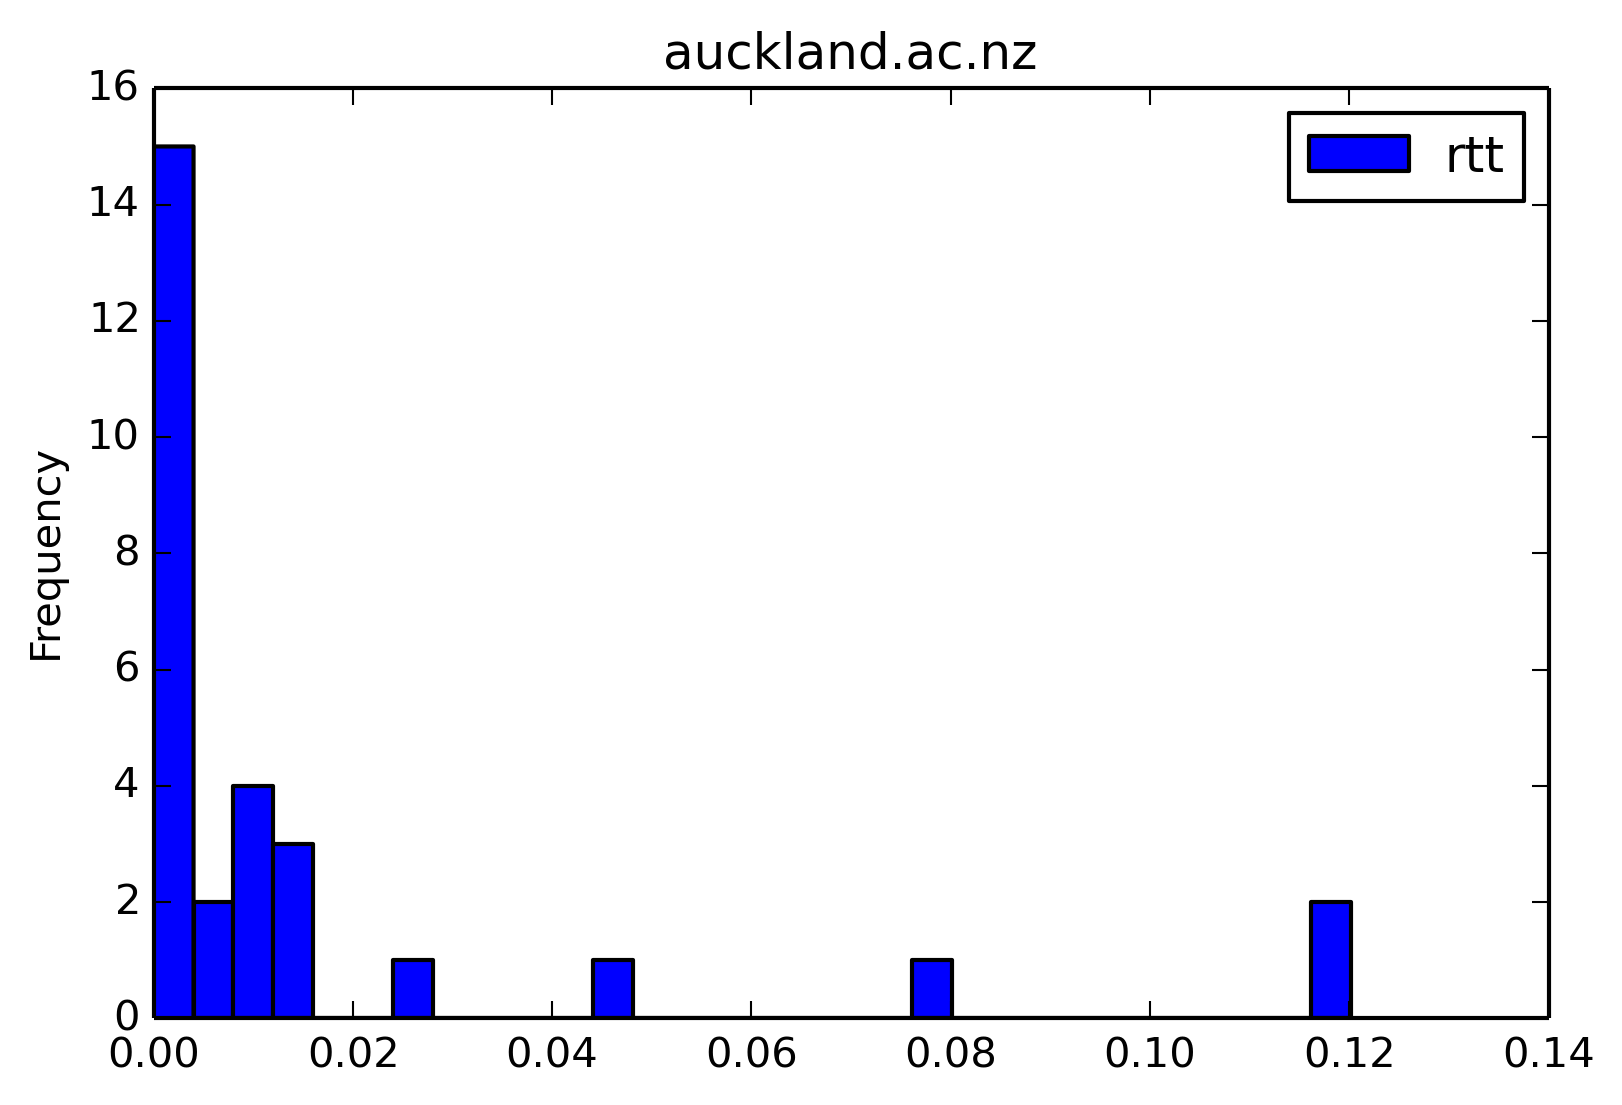
\includegraphics[width=0.45\textwidth]{histogramas_rtt/auckland-ac-nz.png}
  \caption{RTT entre saltos}
  \label{entropia-s}
\end{figure}

\begin{center}
\captionof{table}{Outliers para auckland.ac.nz}
\scalebox{0.8}{
\begin{tabular}{llllr}
\toprule
               &    &               &    &       rtt \\
host & ttl & ip & cc &           \\
\midrule
auckland.ac.nz & 9  & 67.17.94.249 & US &  3.078891 \\
               & 18 & 202.158.194.172 & AU &  3.176235 \\
\bottomrule
\end{tabular}}

\end{center}

\begin{figure}[H]
  \centering
    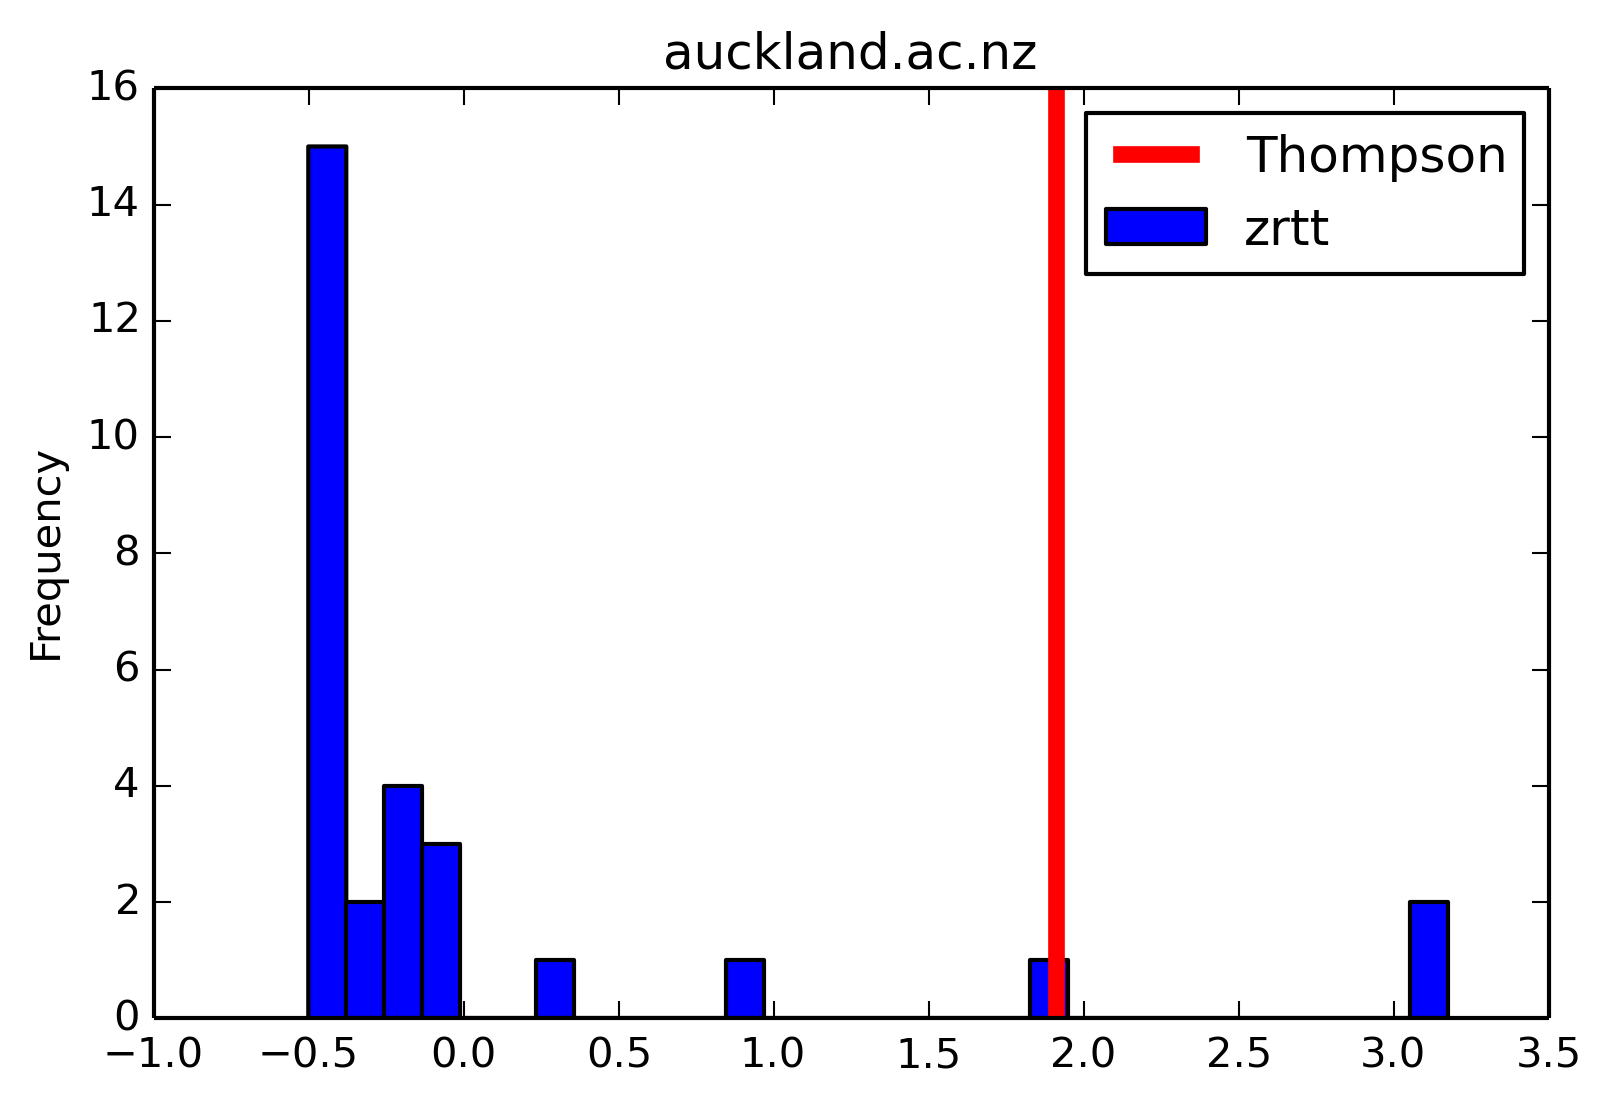
\includegraphics[width=0.45\textwidth]{histogramas_thompson/auckland-ac-nz.png}
  \caption{RTTs Normalizados comparados con el valor Thompson}
  \label{entropia-s}
\end{figure}

\begin{figure}[H]
  \centering
    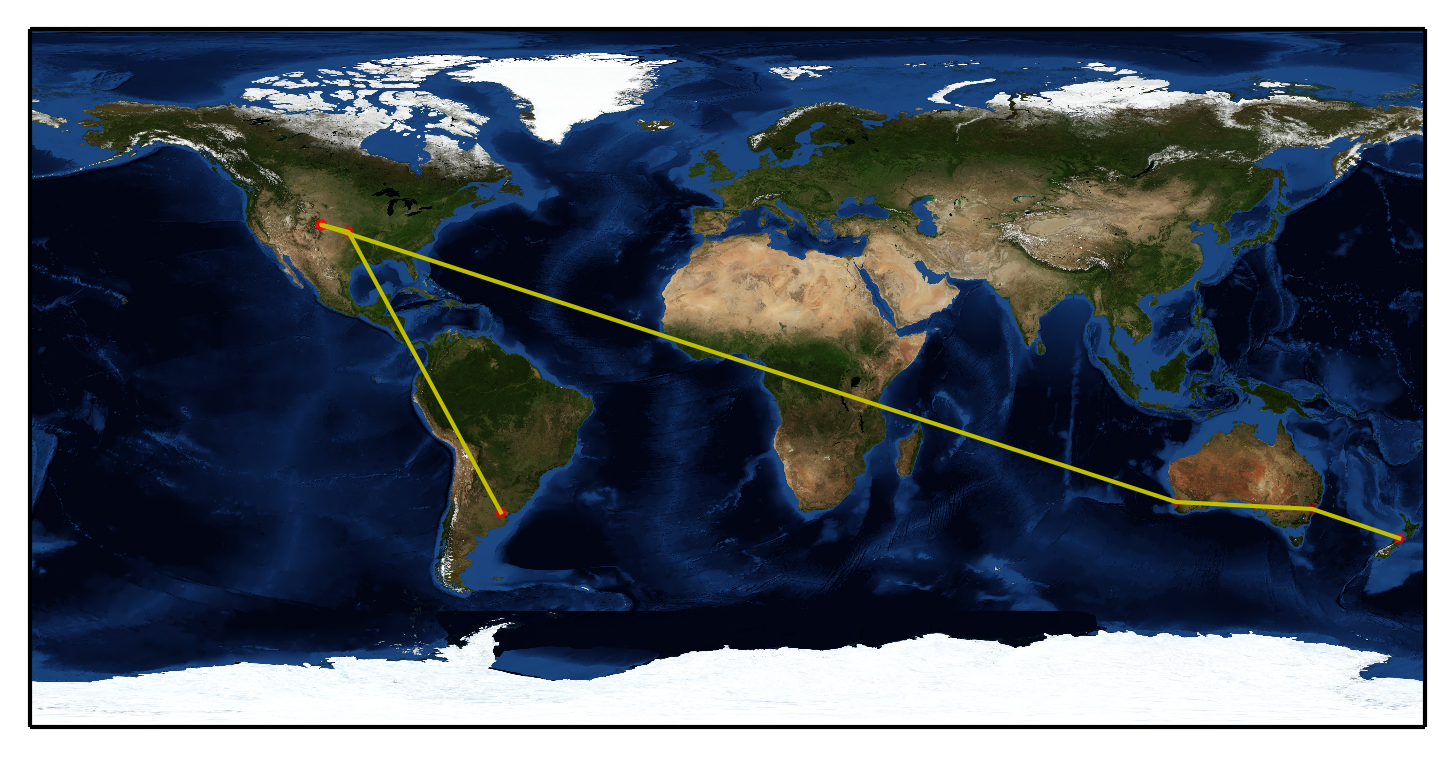
\includegraphics[width=0.45\textwidth]{grafico-rutas/auckland-ac-nz.png}
  \caption{Gráfico de la ruta}
  \label{entropia-s}
\end{figure}




\subsection{Servidor invertisuniversity.ac.in}

\begin{center}
\captionof{table}{rtt promedios entre saltos para invertisuniversity.ac.in}
\scalebox{0.8}{
\begin{tabular}{llllr}
\toprule
                         &    &               &    &       rtt \\
host & ttl & ip & cc &           \\
\midrule
invertisuniversity.ac.in & 1  & empty & empty &  0.000000 \\
                         & 2  & empty & empty &  0.000000 \\
                         & 3  & empty & empty &  0.000000 \\
                         & 4  & empty & empty &  0.000000 \\
                         & 5  & 200.89.161.145 & AR &  0.091815 \\
                         & 6  & 200.89.165.150 & AR&  0.013239 \\
                         & 7  & 185.70.203.20 & IT &  0.016529 \\
                         & 8  & 195.22.209.63 & IT &  0.227124 \\
                         & 9  & 149.3.183.130 & IT &  0.018799 \\
                         & 10 & empty & empty &  0.000000 \\
                         & 11 & 182.79.217.34 & IN &  0.131296 \\
                         & 12 & 202.56.223.241 & IN &  0.022426 \\
                         &    & empty & empty &  0.000000 \\
                         & 13 & 182.79.254.197 & IN &  0.019971 \\
                         & 14 & 125.16.26.235 & IN &  0.007836 \\
                         & 15 & 103.233.124.0 & IN &  0.026050 \\
                         & 16 & 103.233.124.254 & IN &  0.027040 \\
                         & 17 & 103.233.126.5 & IN &  0.017655 \\
                         &    & empty & empty &  0.000000 \\
                         & 18 & 103.233.126.17 & IN &  0.015503 \\
                         & 19 & 103.233.127.47 & IN &  0.011093 \\
                         & 20 & 103.241.180.132 & IN &  0.016200 \\
                         & 21 & 103.241.146.22 & IN &  0.012582 \\
\bottomrule
\end{tabular}}

\end{center}

\begin{center}
\begin{tabular}{p{6.5cm}r}
Porcentaje de saltos que no responden los $Time$ $exceeded$: & \textbf{\%} \\ \\ 
Largo de la ruta en términos de saltos que responden: &\textbf{ saltos} \\ \\
Cantidad de enlaces intercontinentales: & \textbf{} \\ \\
Cantidad de outliers según el método de Cimbala: & \textbf{} \\ \\
\end{tabular}
\end{center}

\begin{figure}[H]
  \centering
    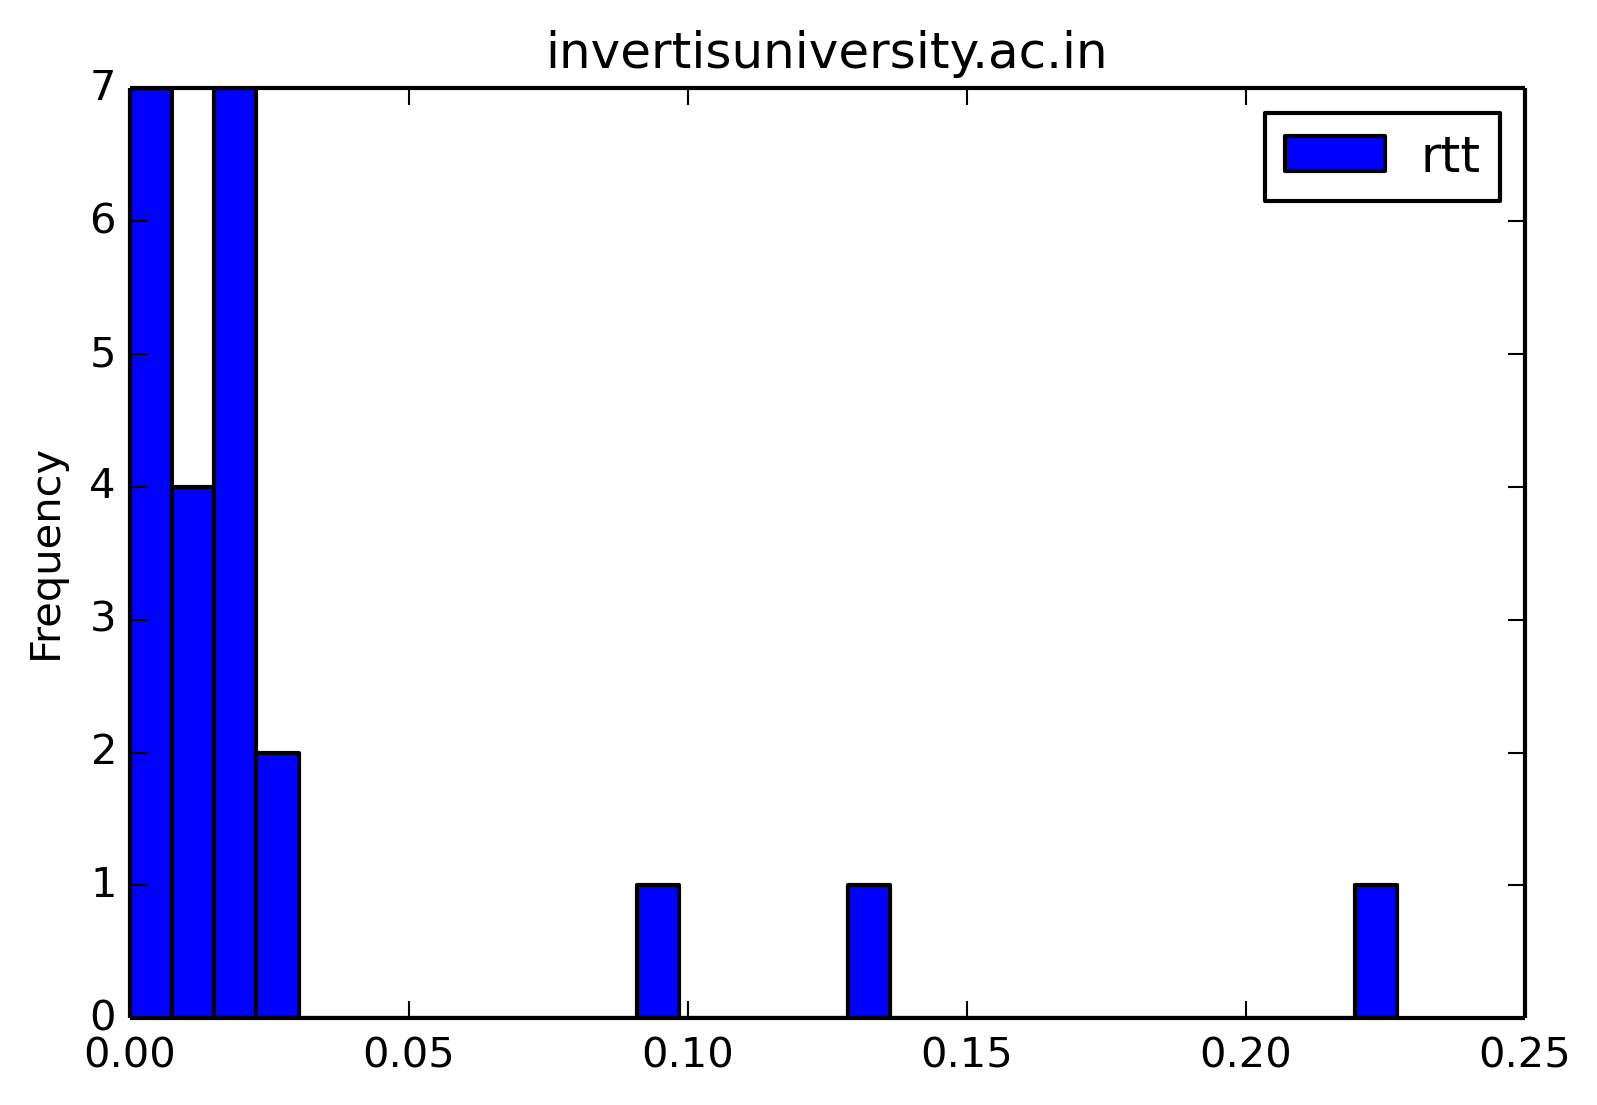
\includegraphics[width=0.45\textwidth]{histogramas_rtt/invertisuniversity-ac-in.png}
  \caption{RTT entre saltos}
  \label{entropia-s}
\end{figure}

\begin{center}
\captionof{table}{Outliers para invertisuniversity.ac.in}
\scalebox{0.8}{
\begin{tabular}{llllr}
\toprule
                         &    &               &    &       rtt \\
host & ttl & ip & cc &           \\
\midrule
invertisuniversity.ac.in & 8  & 195.22.209.63 & IT &  3.734289 \\
                         & 11 & 182.79.217.34 & IN &  1.924863 \\
\bottomrule
\end{tabular}}

\end{center}

\begin{figure}[H]
  \centering
    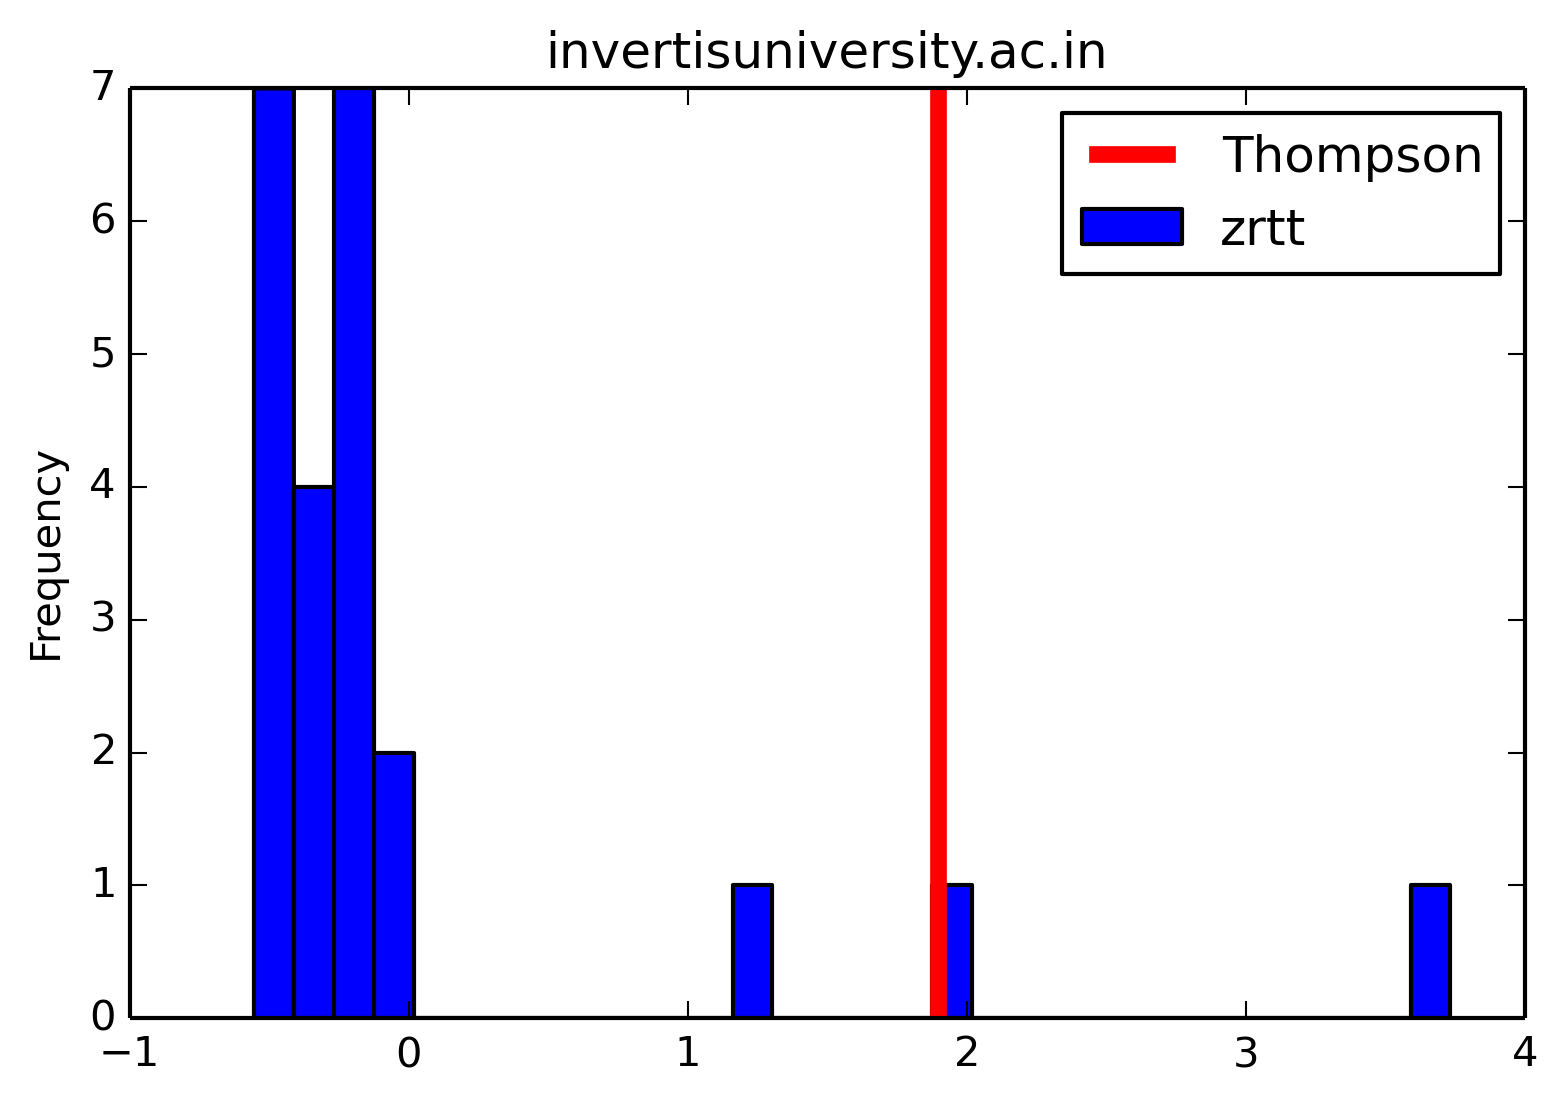
\includegraphics[width=0.45\textwidth]{histogramas_thompson/invertisuniversity-ac-in.png}
  \caption{RTTs Normalizados comparados con el valor Thompson}
  \label{entropia-s}
\end{figure}

\begin{figure}[H]
  \centering
    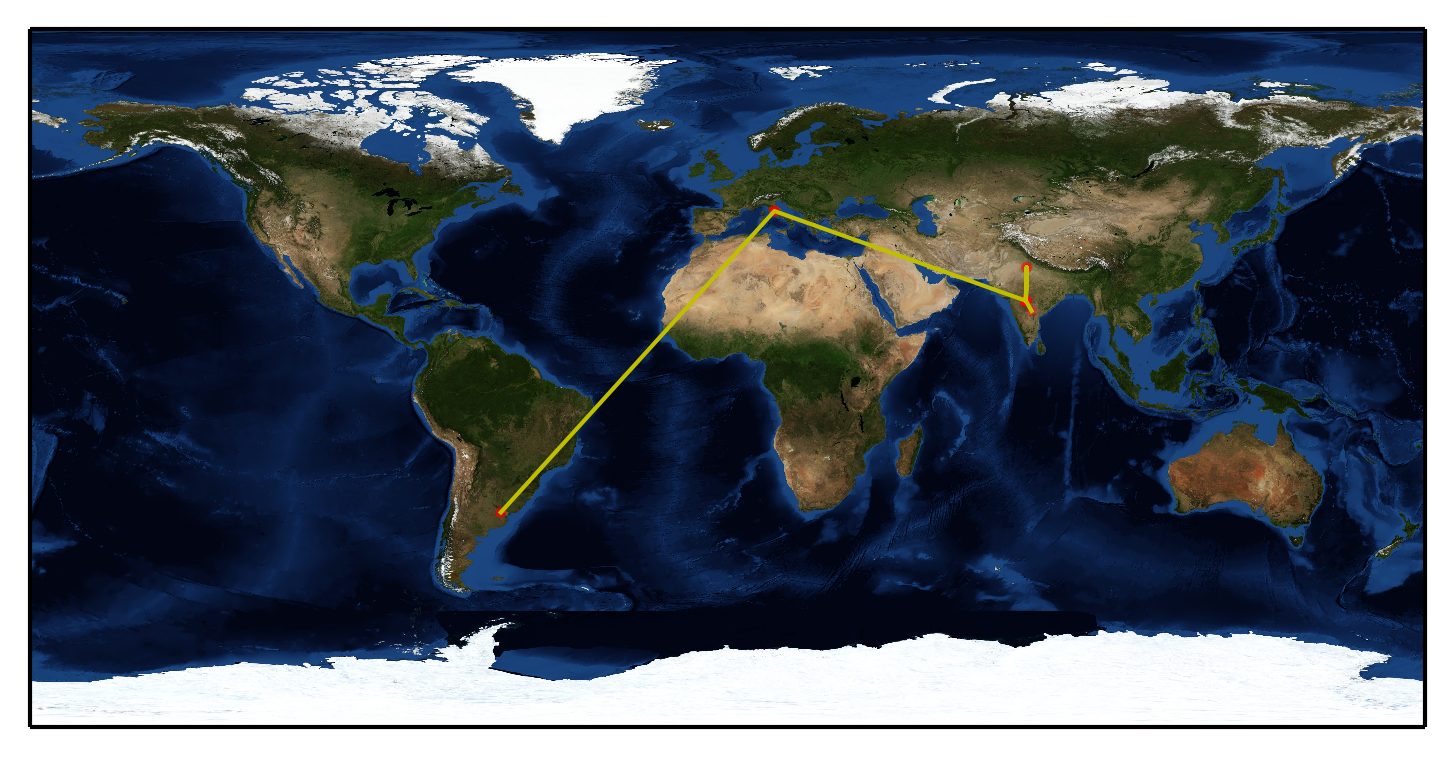
\includegraphics[width=0.45\textwidth]{grafico-rutas/invertisuniversity-ac-in.png}
  \caption{Gráfico de la ruta}
  \label{entropia-s}
\end{figure}




\subsection{Servidor www.uae.ma}

\begin{center}
\captionof{table}{rtt promedios entre saltos para www.uae.ma}
\scalebox{0.8}{
\begin{tabular}{llllr}
\toprule
           &    &              &    &       rtt \\
host & ttl & ip & cc &           \\
\midrule
www.uae.ma & 1  & empty & empty &  0.000000 \\
           & 2  & empty & empty &  0.000000 \\
           & 3  & empty & empty &  0.000000 \\
           & 4  & empty & empty &  0.000000 \\
           & 5  & 200.89.161.129 & AR &  0.074943 \\
           & 6  & 200.89.165.5 & AR &  0.004708 \\
           & 7  & 200.89.165.250 & AR &  0.006304 \\
           & 8  & 195.22.220.102 & IT &  0.005447 \\
           & 9  & 195.22.219.3 & IT &  0.035226 \\
           & 10 &              & IT &  0.010738 \\
           & 11 & 149.3.181.65 & IT &  0.005863 \\
           & 12 & 129.250.2.227 & US &  0.113837 \\
           & 13 & 129.250.2.19 & US &  0.077303 \\
           & 14 & 129.250.4.141 & US &  0.008594 \\
           & 15 & 129.250.6.8 & US &  0.001446 \\
           & 16 & 81.25.207.146 & GB &  0.006293 \\
           & 17 & 50.97.18.211 & US &  0.009113 \\
           & 18 & 50.97.18.249 & US &  0.009749 \\
           & 19 & 159.253.158.131 & NL &  0.004349 \\
           &    & empty & empty &  0.000000 \\
           & 20 & 159.253.148.195 & NL &  0.006204 \\
\bottomrule
\end{tabular}}

\end{center}

\begin{center}
\begin{tabular}{p{6.5cm}r}
Porcentaje de saltos que no responden los $Time$ $exceeded$: & \textbf{25\%} \\ \\ 
Largo de la ruta en términos de saltos que responden: &\textbf{15 saltos} \\ \\
Cantidad de enlaces intercontinentales: & \textbf{4} \\ \\
Cantidad de outliers según el método de Cimbala: & \textbf{} \\ \\
\end{tabular}
\end{center}


\begin{figure}[H]
  \centering
    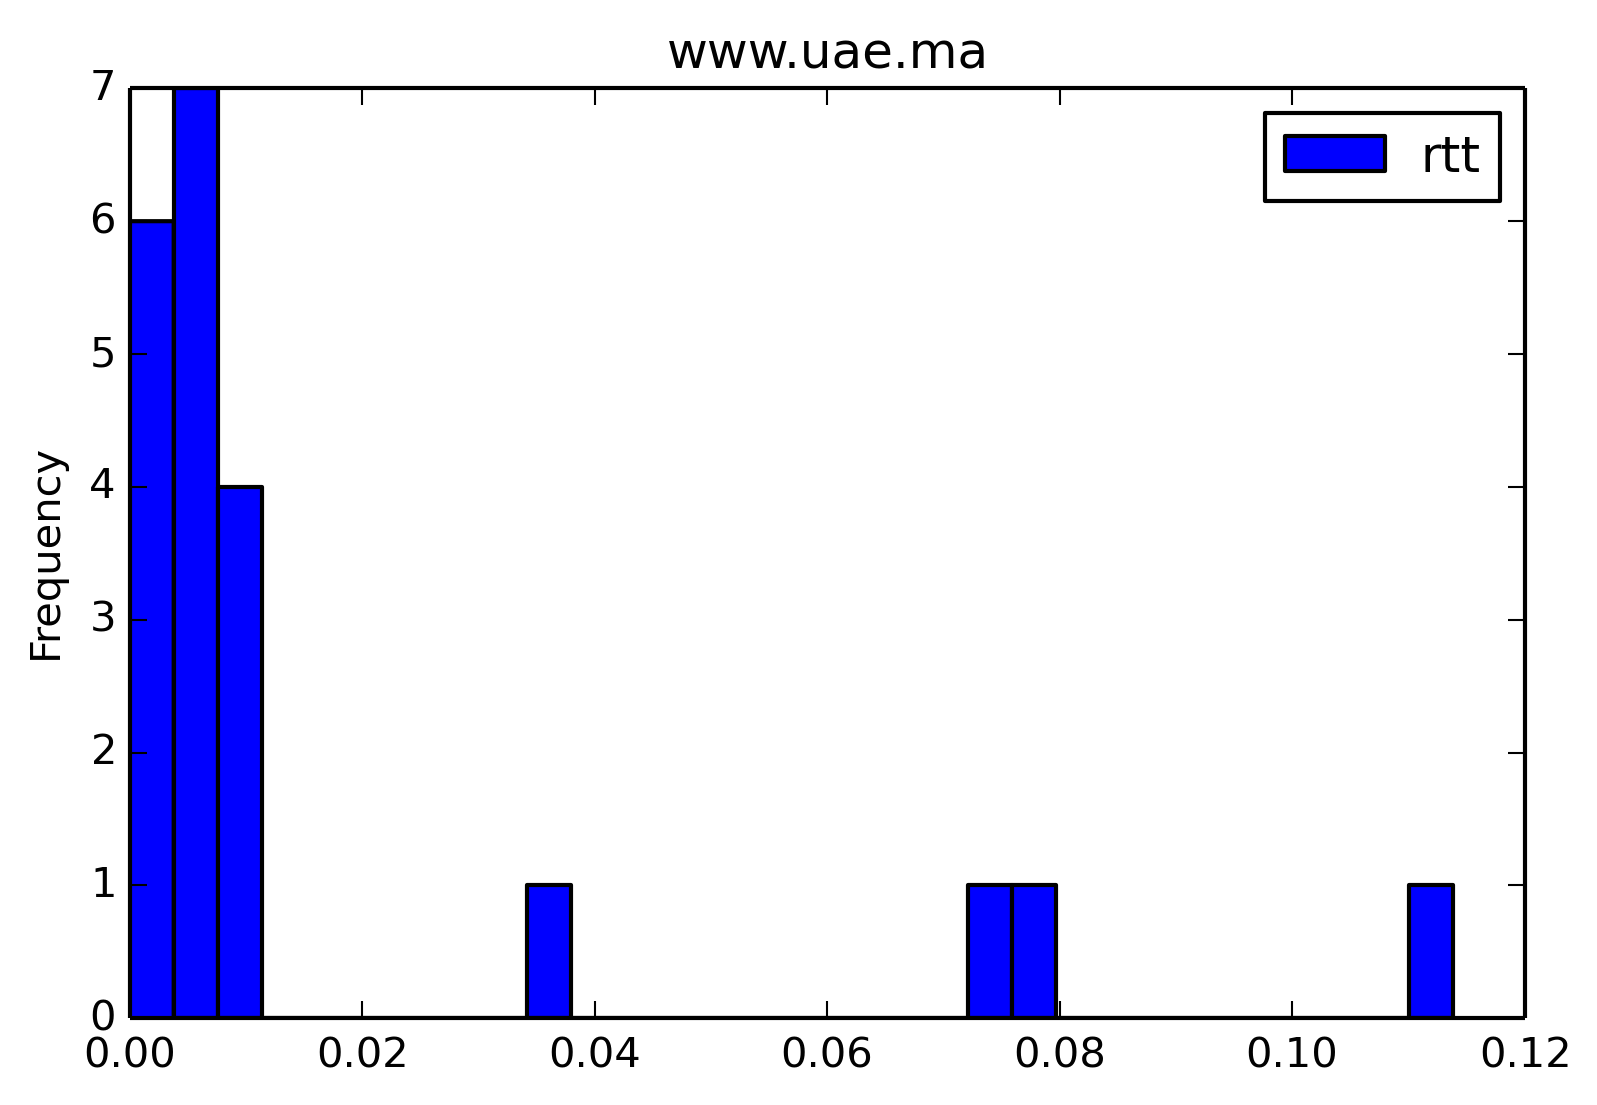
\includegraphics[width=0.45\textwidth]{histogramas_rtt/www-uae-ma.png}
  \caption{RTT entre saltos}
  \label{entropia-s}
\end{figure}

\begin{center}
\captionof{table}{Outliers para www.uae.ma}
\scalebox{0.8}{
\begin{tabular}{llllr}
\toprule
           &    &              &    &       rtt \\
host & ttl & ip & cc &           \\
\midrule
www.uae.ma & 12 & 129.250.2.227 & US &  3.065712 \\
           & 13 & 129.250.2.19 & US &  1.895807 \\
\bottomrule
\end{tabular}}

\end{center}

\begin{figure}[H]
  \centering
    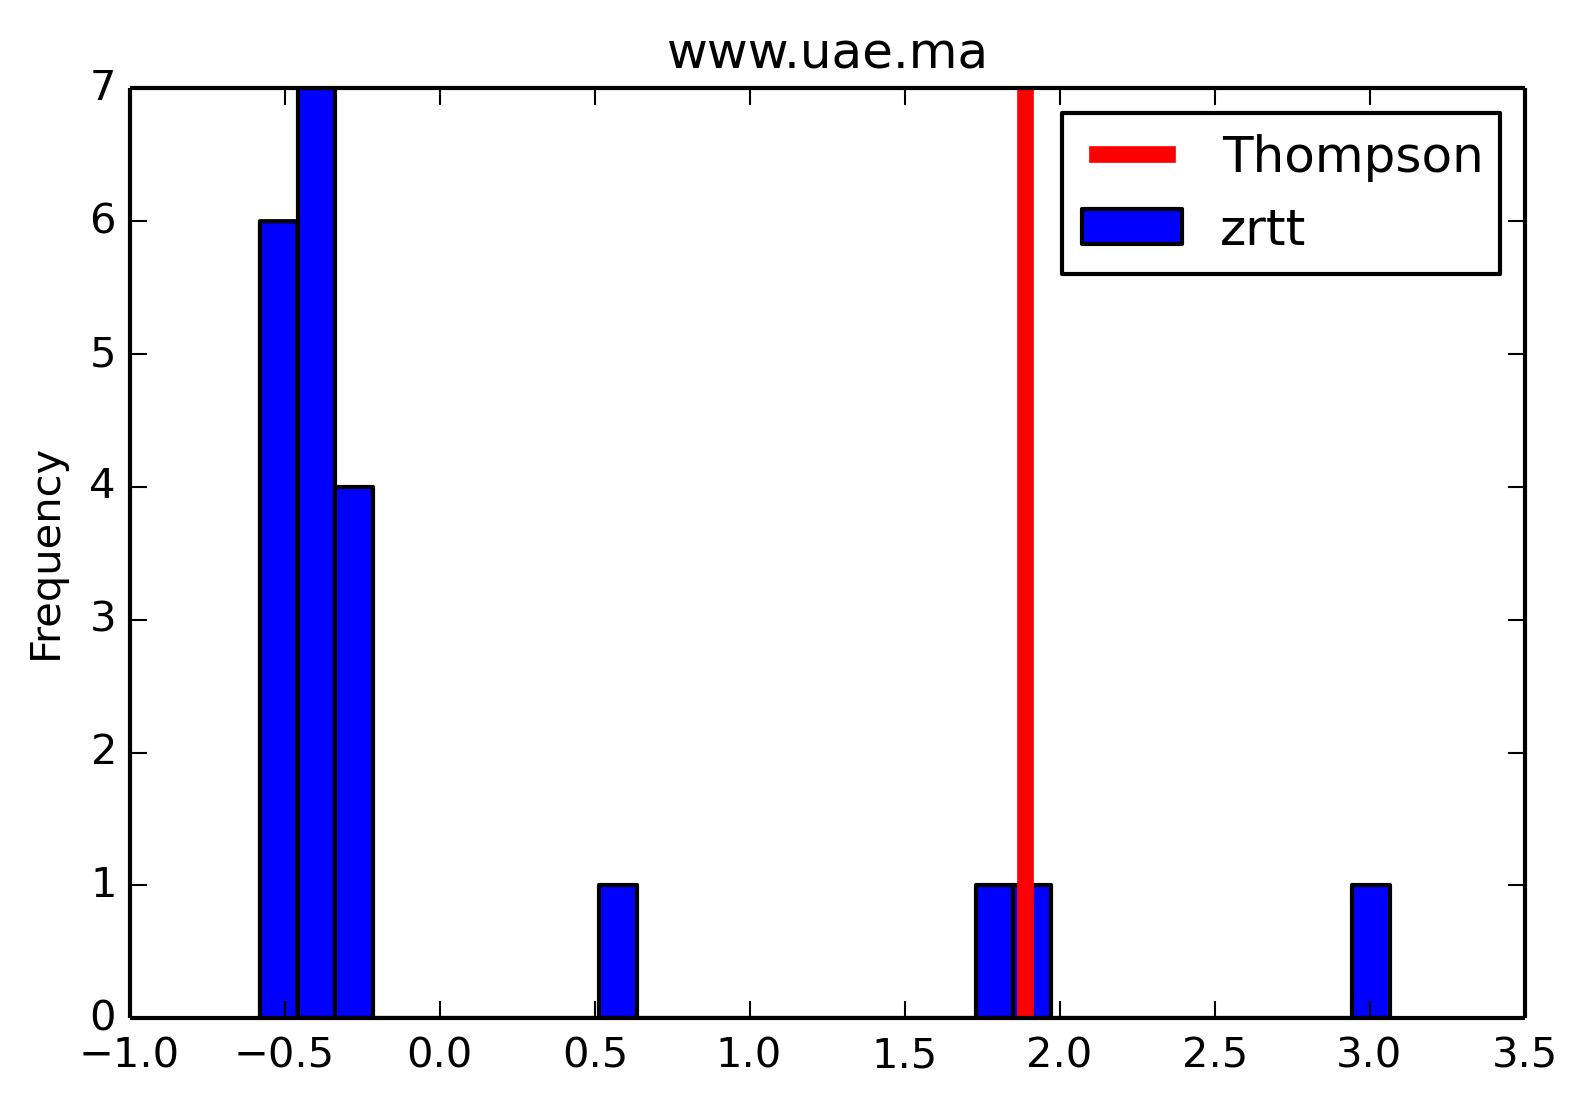
\includegraphics[width=0.45\textwidth]{histogramas_thompson/www-uae-ma.png}
  \caption{RTTs Normalizados comparados con el valor Thompson}
  \label{entropia-s}
\end{figure}

\begin{figure}[H]
  \centering
    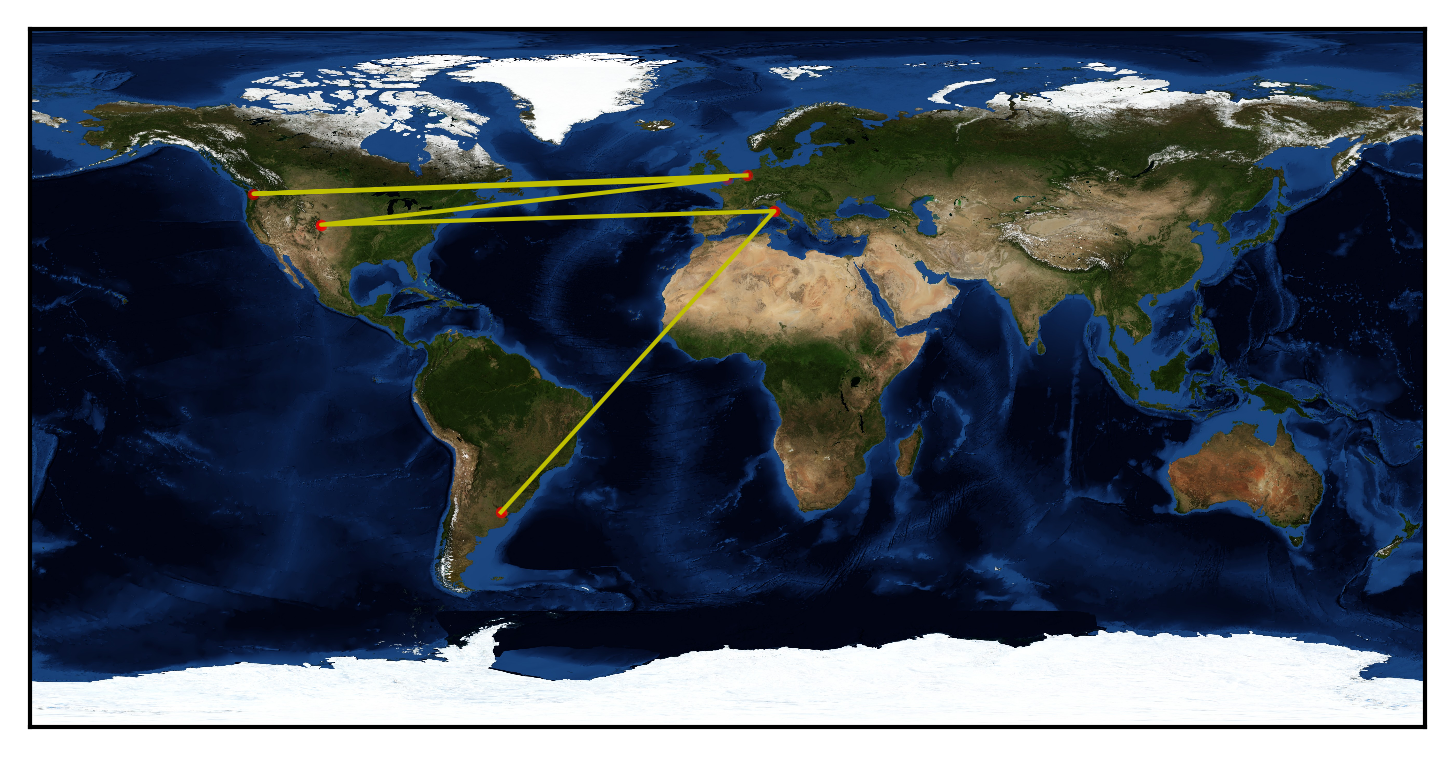
\includegraphics[width=0.45\textwidth]{grafico-rutas/www-uae-ma.png}
  \caption{Gráfico de la ruta}
  \label{entropia-s}
\end{figure}




\subsection{Servidor bifrost.is}

\begin{center}
\captionof{table}{rtt promedios entre saltos para bifrost.is}
\scalebox{0.8}{
\begin{tabular}{llllr}
\toprule
           &    &               &    &       rtt \\
host & ttl & ip & cc &           \\
\midrule
bifrost.is & 1  & empty & empty &  0.000000 \\
           & 2  & empty & empty &  0.000000 \\
           & 3  & empty & empty &  0.000000 \\
           & 4  & empty & empty &  0.000000 \\
           & 5  & 200.89.161.133 & AR &  0.077077 \\
           & 6  & 200.89.165.130 & AR &  0.004429 \\
           & 7  & 200.89.165.222 & AR &  0.006434 \\
           & 8  & 185.70.203.32 & IT &  0.003869 \\
           & 9  & 89.221.41.171 & IT &  0.128319 \\
           & 10 &               & IT &  0.006943 \\
           & 11 & 154.54.9.17 & US &  0.005663 \\
           & 12 & 154.54.24.233 & US &  0.003648 \\
           & 13 & 154.54.24.197 & US &  0.011277 \\
           & 14 & 154.54.24.221 & US &  0.009189 \\
           & 15 & 154.54.40.109 & US &  0.007895 \\
           & 16 & 154.54.42.86 & US &  0.091001 \\
           & 17 & 154.54.57.162 & US &  0.008998 \\
           & 19 & 149.6.98.110 & US &  0.013127 \\
           & 20 & 31.15.113.2 & IS &  0.013911 \\
           & 21 & 31.15.113.1 & IS &  0.008186 \\
           & 22 & 31.15.115.41 & IS &  0.007656 \\
           & 23 & 176.10.35.233 & IS &  0.031531 \\
           & 24 & 176.10.35.234 & IS &  0.004080 \\
           & 25 & 185.118.33.147 & IS &  0.007998 \\
\bottomrule
\end{tabular}}

\end{center}

\begin{center}
\begin{tabular}{p{6.5cm}r}
Porcentaje de saltos que no responden los $Time$ $exceeded$: & \textbf{17\%} \\ \\ 
Largo de la ruta en términos de saltos que responden: &\textbf{20 saltos} \\ \\
Cantidad de enlaces intercontinentales: & \textbf{4} \\ \\
Cantidad de outliers según el método de Cimbala: & \textbf{} \\ \\
\end{tabular}
\end{center}

\begin{figure}[H]
  \centering
    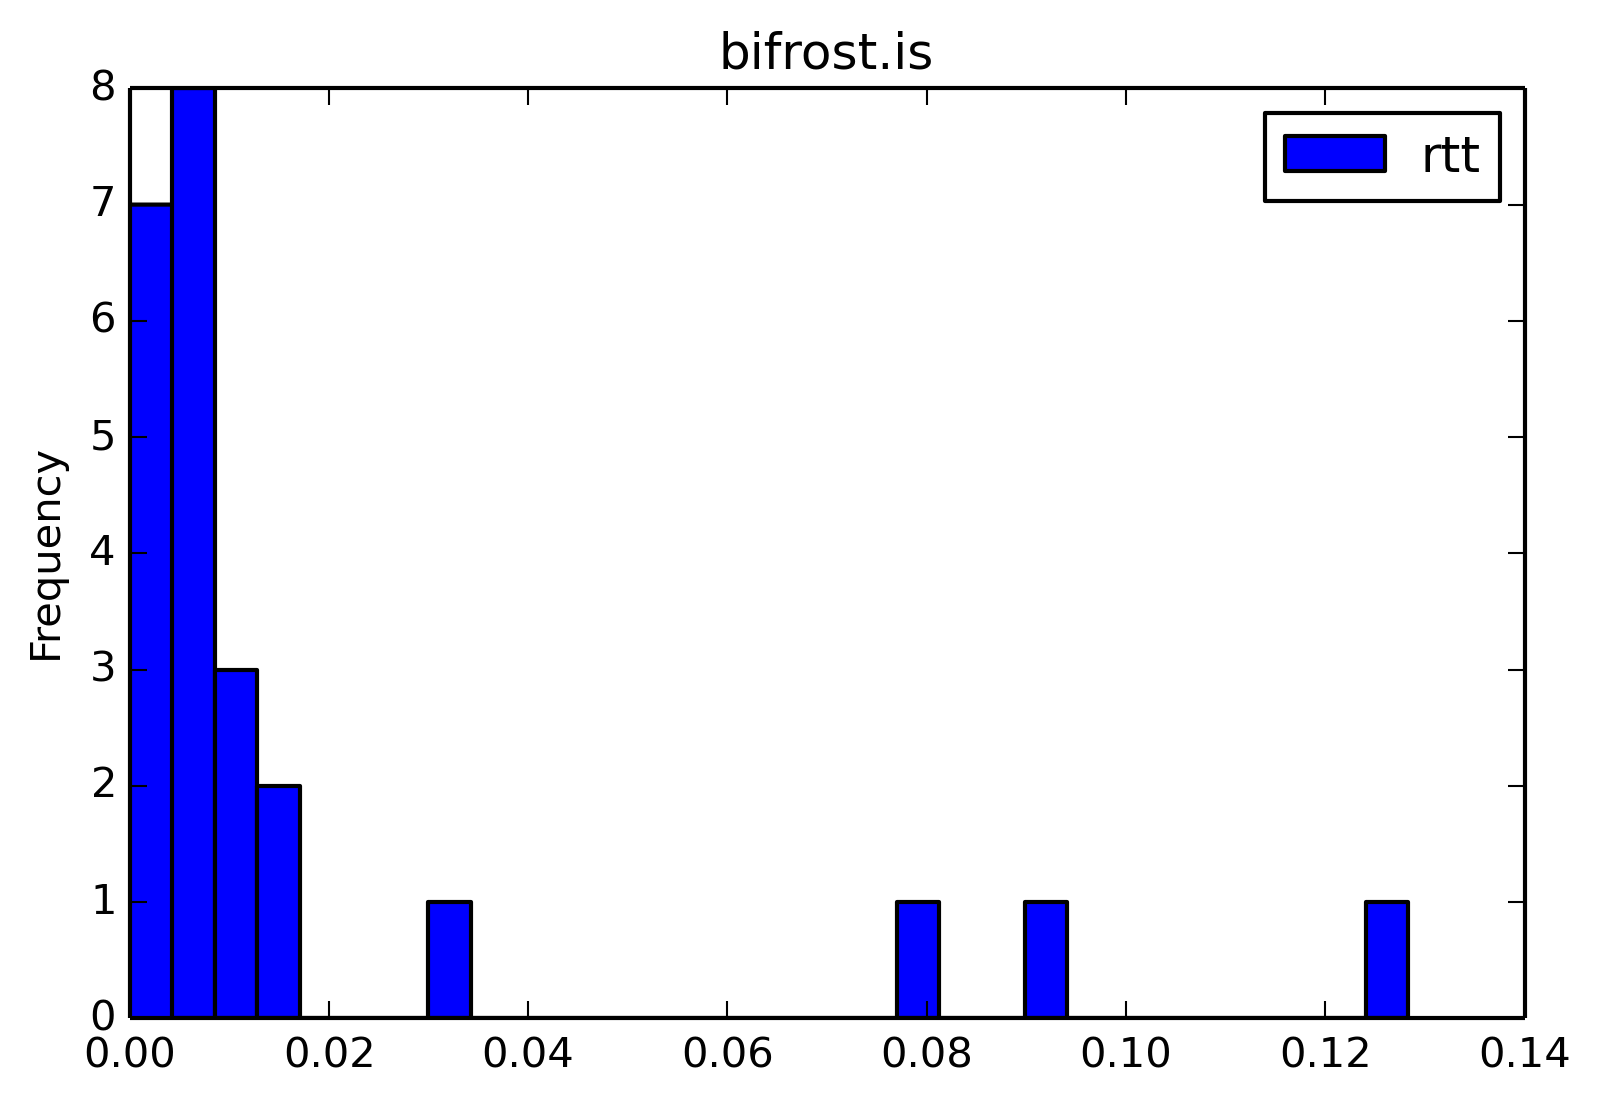
\includegraphics[width=0.45\textwidth]{histogramas_rtt/bifrost-is.png}
  \caption{RTT entre saltos}
  \label{entropia-s}
\end{figure}

\begin{center}
\captionof{table}{Outliers para bifrost.is}
\scalebox{0.8}{
\begin{tabular}{llllr}
\toprule
           &    &               &    &       rtt \\
host & ttl & ip & cc &           \\
\midrule
bifrost.is & 9  & 89.221.41.171 & IT &  3.369697 \\
           & 16 & 154.54.42.86 & US &  2.221474 \\
\bottomrule
\end{tabular}}

\end{center}

\begin{figure}[H]
  \centering
    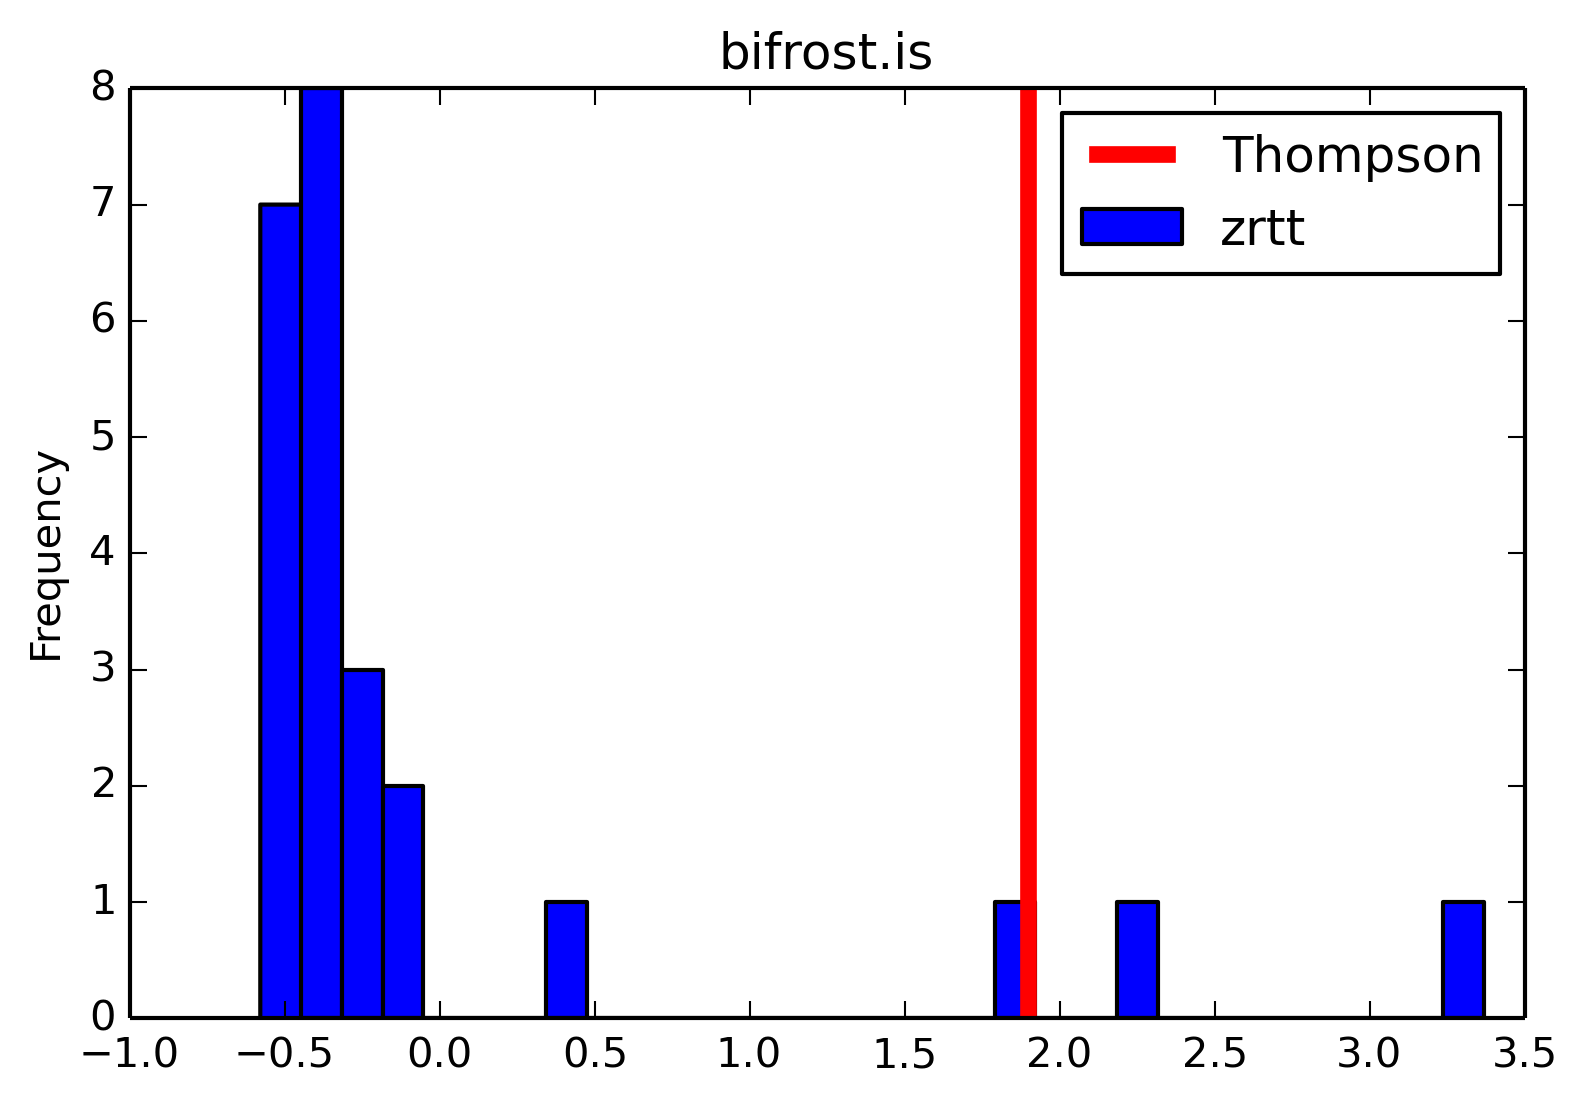
\includegraphics[width=0.45\textwidth]{histogramas_thompson/bifrost-is.png}
  \caption{RTTs Normalizados comparados con el valor Thompson}
  \label{entropia-s}
\end{figure}

\begin{figure}[H]
  \centering
    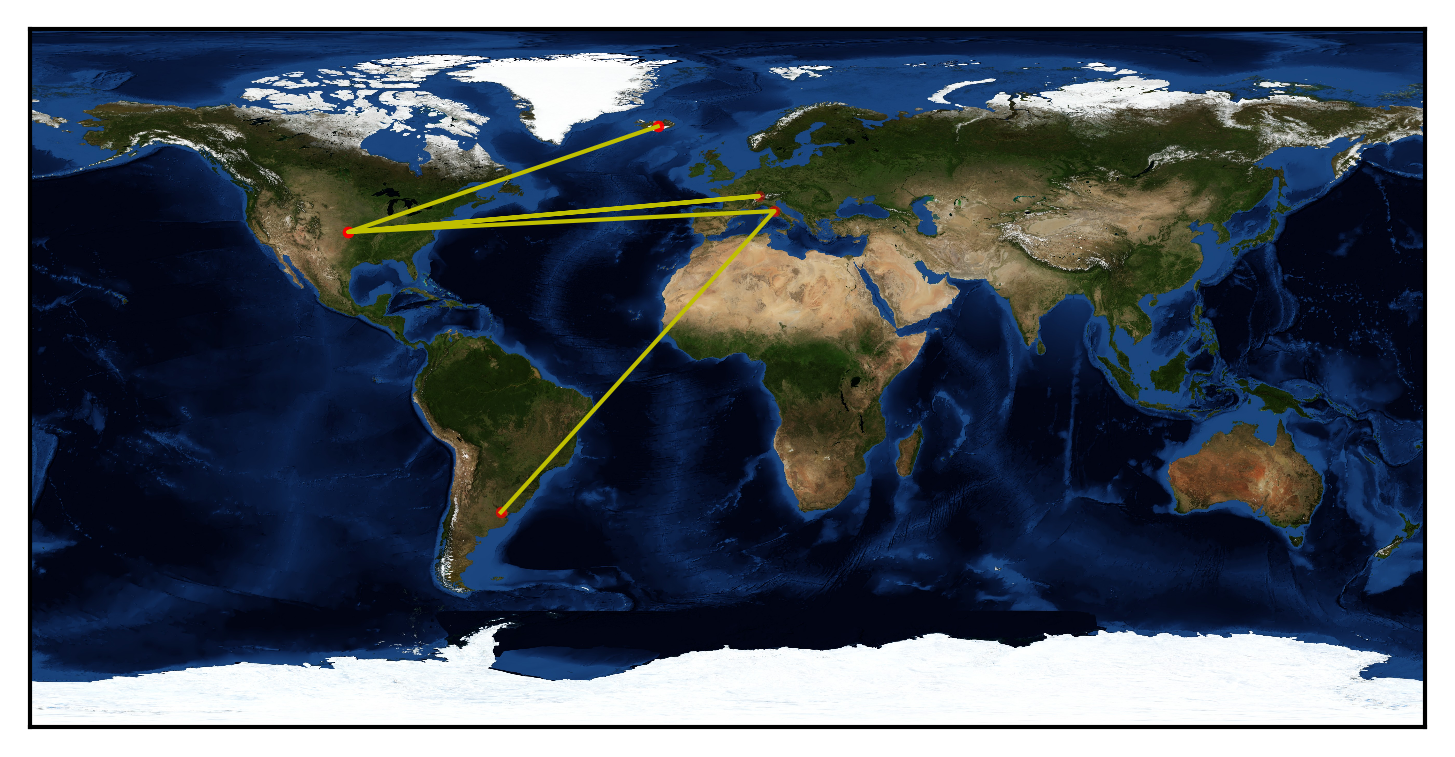
\includegraphics[width=0.45\textwidth]{grafico-rutas/bifrost-is.png}
  \caption{Gráfico de la ruta}
  \label{entropia-s}
\end{figure}




\subsection{Servidor birmingham.ac.uk}

\begin{center}
\captionof{table}{rtt promedios entre saltos para birmingham.ac.uk}
\scalebox{0.8}{
\begin{tabular}{llllr}
\toprule
                 &    &             &    &       rtt \\
host & ttl & ip & cc &           \\
\midrule
birmingham.ac.uk & 1  & empty & empty &  0.000000 \\
                 & 2  & empty & empty &  0.000000 \\
                 & 3  & empty & empty &  0.000000 \\
                 & 4  & empty & empty &  0.000000 \\
                 & 5  & 200.89.161.85 & AR &  0.074961 \\
                 & 6  & 200.89.165.1 & AR &  0.004908 \\
                 & 7  & 200.89.165.250 & AR &  0.007433 \\
                 & 8  & empty & empty &  0.000000 \\
                 & 9  & 67.17.99.233 & US &  0.124818 \\
                 & 10 & empty & empty &  0.000000 \\
                 & 11 & empty & empty &  0.000000 \\
                 & 12 & 212.187.139.166 & GB &  0.090183 \\
                 & 13 & 146.97.33.2 & GB &  0.006402 \\
                 & 14 & 146.97.33.22 & GB &  0.006861 \\
                 & 15 & 146.97.37.154 & GB &  0.010930 \\
                 & 16 & 193.62.80.154 & GB &  0.005032 \\
                 & 17 & 193.62.80.174 & GB &  0.005705 \\
                 & 18 & 193.63.208.142 & GB &  0.007928 \\
                 & 19 & empty & empty &  0.000000 \\
\bottomrule
\end{tabular}}

\end{center}

\begin{center}
\begin{tabular}{p{6.5cm}r}
Porcentaje de saltos que no responden los $Time$ $exceeded$: & \textbf{62\%} \\ \\ 
Largo de la ruta en términos de saltos que responden: &\textbf{11 saltos} \\ \\
Cantidad de enlaces intercontinentales: & \textbf{1} \\ \\
Cantidad de outliers según el método de Cimbala: & \textbf{3} \\ \\
\end{tabular}
\end{center}

\begin{figure}[H]
  \centering
    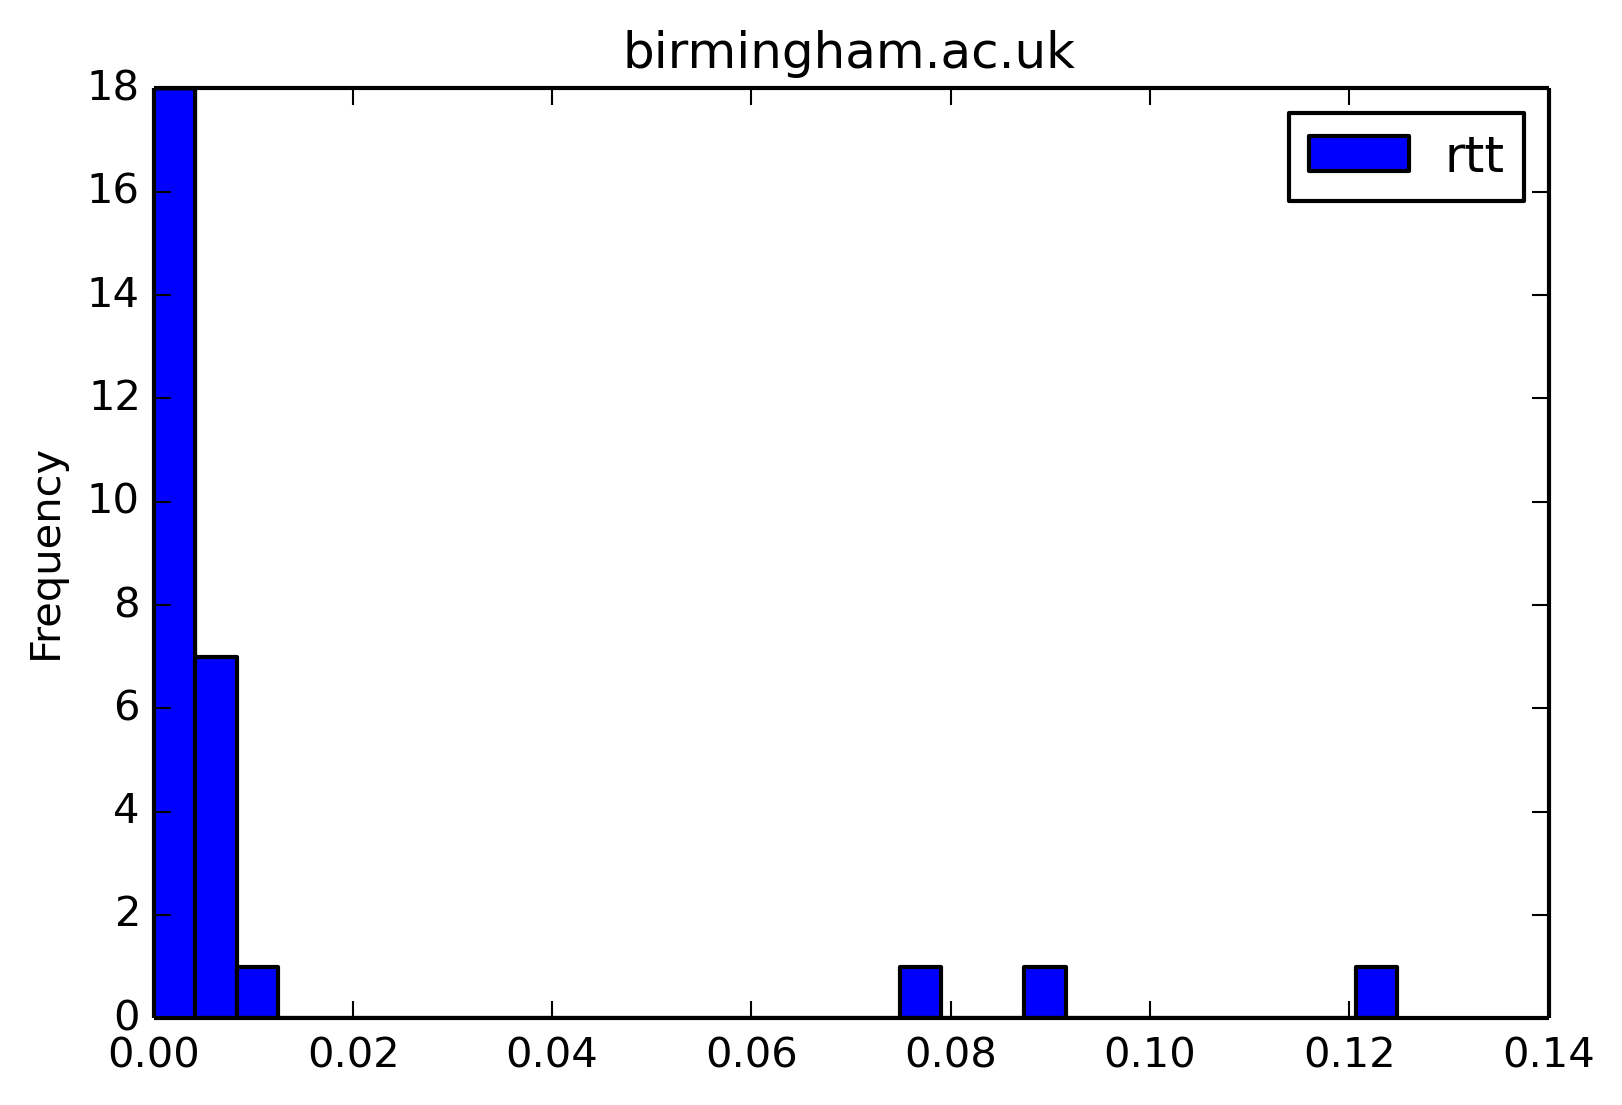
\includegraphics[width=0.45\textwidth]{histogramas_rtt/birmingham-ac-uk.png}
  \caption{RTT entre saltos}
  \label{entropia-s}
\end{figure}

\begin{center}
\captionof{table}{Outliers para birmingham.ac.uk}
\scalebox{0.8}{
\begin{tabular}{llllr}
\toprule
                 &    &             &    &       rtt \\
host & ttl & ip & cc &           \\
\midrule
birmingham.ac.uk & 5  & 200.89.161.85 & AR &  2.084216 \\
                 & 9  & 67.17.99.233 & US &  3.732069 \\
                 & 12 & 212.187.139.166 & GB &  2.587332 \\
\bottomrule
\end{tabular}}

\end{center}

\begin{figure}[H]
  \centering
    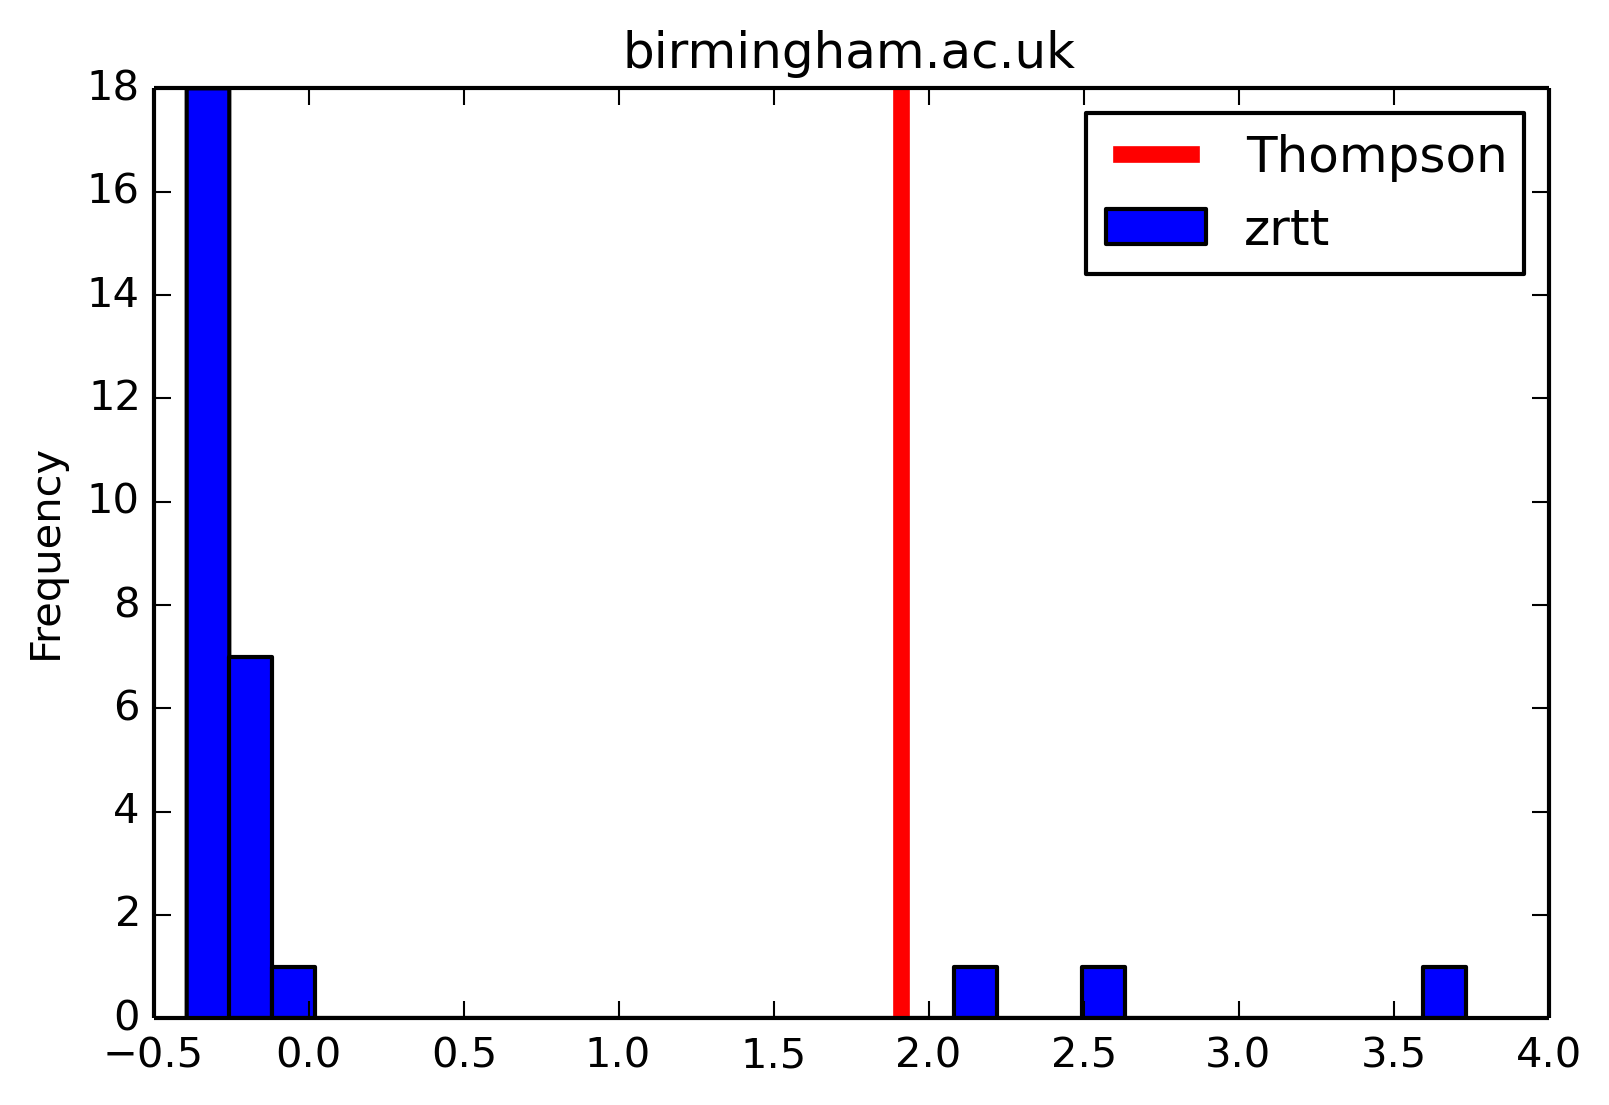
\includegraphics[width=0.45\textwidth]{histogramas_thompson/birmingham-ac-uk.png}
  \caption{RTTs Normalizados comparados con el valor Thompson}
  \label{entropia-s}
\end{figure}

\begin{figure}[H]
  \centering
    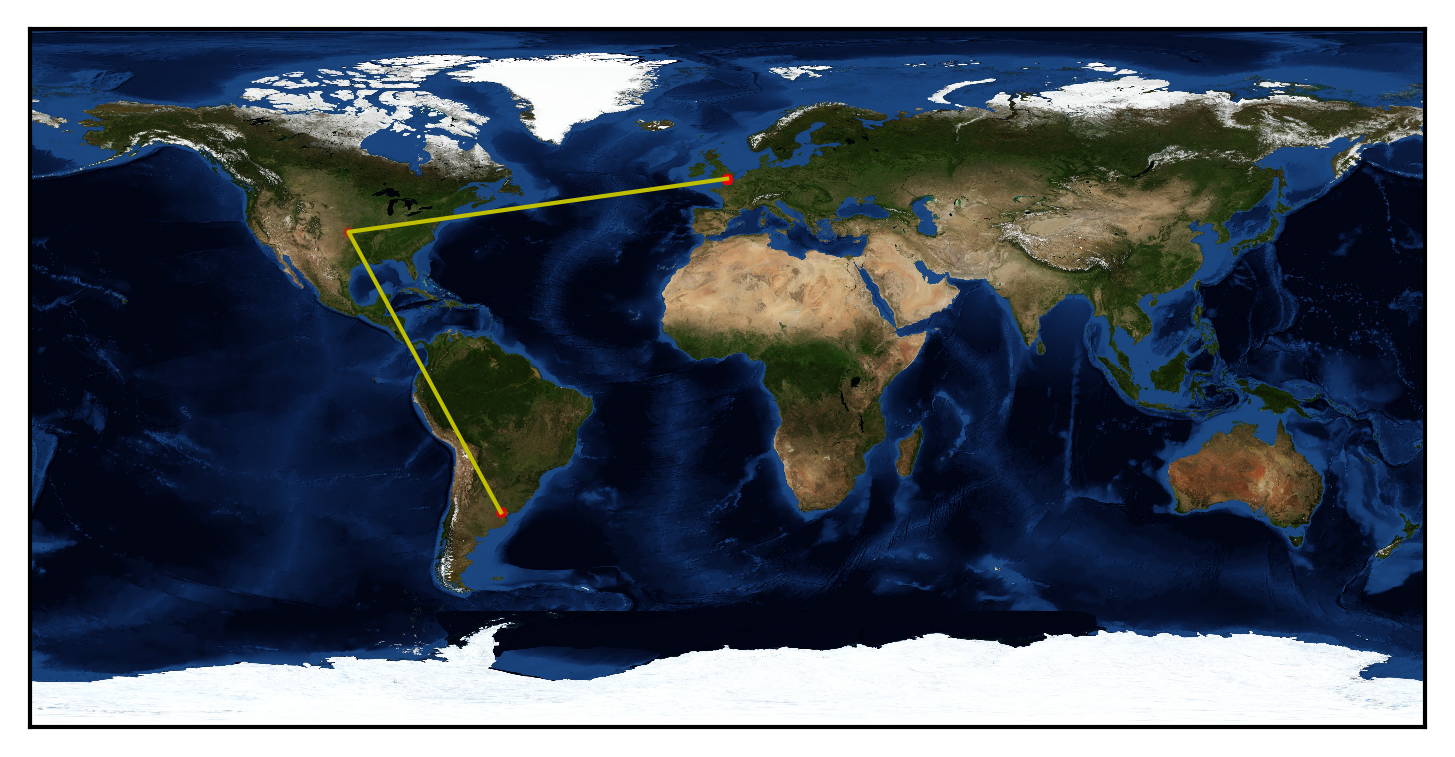
\includegraphics[width=0.45\textwidth]{grafico-rutas/birmingham-ac-uk.png}
  \caption{Gráfico de la ruta}
  \label{entropia-s}
\end{figure}